% file: DGDT_dump.tex
% Differential Geometry, Differential Topology, in unconventional ``grande'' format; fitting a widescreen format
% 
% github        : ernestyalumni
% linkedin      : ernestyalumni 
% wordpress.com : ernestyalumni
%
% This code is open-source, governed by the Creative Common license.  Use of this code is governed by the Caltech Honor Code: ``No member of the Caltech community shall take unfair advantage of any other member of the Caltech community.'' 
% 

\documentclass[10pt]{amsart}
\pdfoutput=1
\usepackage{mathtools,amssymb,lipsum,caption}

\usepackage{graphicx}
\usepackage{hyperref}
\usepackage[utf8]{inputenc}
\usepackage{listings}
\usepackage[table]{xcolor}
\usepackage{pdfpages}
%\usepackage[version=3]{mhchem}
\usepackage{mhchem}

\usepackage{tikz}
\usetikzlibrary{matrix,arrows}

\usepackage{multicol}

\hypersetup{colorlinks=true,citecolor=[rgb]{0,0.4,0}}

\oddsidemargin=15pt
\evensidemargin=5pt
\hoffset-45pt
\voffset-55pt
\topmargin=-4pt
\headsep=5pt
\textwidth=1120pt
\textheight=595pt
\paperwidth=1200pt
\paperheight=700pt
\footskip=40pt








\newtheorem{theorem}{Theorem}
\newtheorem{corollary}{Corollary}
%\newtheorem*{main}{Main Theorem}
\newtheorem{lemma}{Lemma}
\newtheorem{proposition}{Proposition}

\newtheorem{definition}{Definition}
\newtheorem{remark}{Remark}

\newenvironment{claim}[1]{\par\noindent\underline{Claim:}\space#1}{}
\newenvironment{claimproof}[1]{\par\noindent\underline{Proof:}\space#1}{\hfill $\blacksquare$}

%This defines a new command \questionhead which takes one argument and
%prints out Question #. with some space.
\newcommand{\questionhead}[1]
  {\bigskip\bigskip
   \noindent{\small\bf Question #1.}
   \bigskip}

\newcommand{\problemhead}[1]
  {
   \noindent{\small\bf Problem #1.}
   }

\newcommand{\exercisehead}[1]
  { \smallskip
   \noindent{\small\bf Exercise #1.}
  }

\newcommand{\solutionhead}[1]
  {
   \noindent{\small\bf Solution #1.}
   }


\title{The Differential Geometry Differential Topology Dump}
\author{Ernest Yeung \href{mailto:ernestyalumni@gmail.com}{ernestyalumni@gmail.com}}
\date{28 juillet 2016}
\keywords{Differential Geometry, Differential Topology}
\begin{document}

\definecolor{darkgreen}{rgb}{0,0.4,0}
\lstset{language=Python,
 frame=bottomline,
 basicstyle=\scriptsize,
 identifierstyle=\color{blue},
 keywordstyle=\bfseries,
 commentstyle=\color{darkgreen},
 stringstyle=\color{red},
 }
%\lstlistoflistings

\maketitle



\begin{multicols*}{2}

  
\setcounter{tocdepth}{1}
\tableofcontents



\begin{abstract}
Everything about Differential Geometry, Differential Topology

\end{abstract}

\part{Combinatorics, Probability Theory}

\begin{theorem}[4.2. of Feller (1968)  \cite{Fell1968}]
	Let $r_1,\dots r_k \in \mathbb{Z}$, s.t. $r_1 + r_2 + \dots + r_k = n$;, $r_i \geq 0$.  

Let 
\begin{equation}
\frac{ N! }{r_1! r_2! \dots r_k!} = 
\end{equation}
number of ways in which $n$ elemnts can be divided into $k$ ordered parts (partitioned into $k$ subpopulations).  cf. Eq. (4.7) of Feller (1968)  \cite{Fell1968}.  

Note that the order of the subpopulations is essential in the sense that ($r_1 = 2,r_2 =3$) and ($r_1=3,r_2=2$) represent different partitions.  However, no attention is paid to the order within the groups.  

\end{theorem}
\begin{proof}
\begin{equation}
\binom{n}{r_1} \binom{n-r_1}{r_2} \binom{n-r_1-r_2}{r_3} \dots \binom{n-r_1-\dots - r_{k-2} }{ r_{k-1} } = \frac{n!}{ r_1! r_2! \dots r_k! }
\end{equation}
i.e. in order to effect the desired partition, we have to select $r_1$ elementsout of $n$, remaining $n-r_1$ elements select a second group of size $r_2$, etc.  After forming the $(k-1)$st group there remains $n-r_1 -r_2 - \dots - r_{k-1} = r_k$ elements, and these form the last group.  
\end{proof}

cf. pp. 37 of Feller (1968)  \cite{Fell1968}
Examples.  (g) Bridge.  32 cards are partitioned into 4 equal groups $\to 52!/(13!)^4$.  

Probability each player has an ace (?).  

The 4 aces can be ordered in $4! = 24$ ways, each order presents 1 possibility of giving 1 ace to each player.  \\
Remaining 48 cards distributed $(48!)/( 12!)^4$ ways.  

\[
\to p = 24 \frac{ 48!}{ (12!)^4 } / \frac{ 52!}{ (13!)^4}
\]

(h) A throw of 12 dice $\to  6^{12}$ different outcomes total.  Event each face appears twice can occur in as many ways as 12 dice can be arranged in 6 groups of 2 each.  
\[
\frac{12!}{(2!)^6} / \frac{ 52!}{ (13!)^4} 
\]

\subsubsection{Application to Occupancy Problems; binomial coefficients}

cf. Sec. 5 Application to Occupancy Problems of Feller (1968)  \cite{Fell1968}.  

Consider randomly placing $r$ balls intos $n$ cells.  

Let $r_k = $ occupancy number $=$ number of balls in $k$th cell.  

Every $n$-tuple of integers satisfying $r_1 + r_2 + \dots + r_n = r$;  $r_k \geq 0$.  describes a possible configuration of occupancy numbers.  

With indistinguishable balls 2 distributions are distinguishable only if the corresponding $n$-tuples ($r_1,\dots r_n$) are not identical.  

\begin{enumerate}
\item[(i)] number of distinguishable distributions is 
\begin{equation}
A_{r,n} = \binom{n+r-1}{r} = \binom{n+r-1}{n-1}  
\end{equation} cf. Eq. (5.2) of Feller (1968)  \cite{Fell1968}
\item[(ii)]  number of distinguishable distributions in which no cell remains empty is $\binom{r-1}{n-1}$.  
\end{enumerate}

\begin{proof}
Represent balls by stars, indicate $n$ cells by $n$ spaces between $n+1$ bars.  e.g. $\begin{aligned} & \quad \\ 
& r= 8 \text{ balls } \\
& n = 6 \text{ cells } \end{aligned}$.  

\[
\begin{aligned}
	& 3 	  & 1   & 0 & 0 & 0 & 4 \\
	& | * * * & | * & | & |   & | & | **** |  
\end{aligned}
\]

Such a symbol necessarily starts and ends with a bar, but remaining $n-1$ bars and $r$ starts appear in an arbitrary order.  In this way, it becomes apparent that the number of distinguishable distributions equals the number of ways of selecting.  

$r$ places out of $n+r-1$, $\frac{ (n+r-1)! }{ (n-1)! r!} = \binom{n-1+r}{r} $  

\[
\begin{aligned}
	& | | | | \dots | | \qquad \, n+1 \text{ bars } \\ 
	& * * * \dots * * \qquad \, r \text{ stars leave } r-1 \text{ spaces }
\end{aligned}
\]

Condition that no cell be empty imposes the restriction that no 2 bars be adjacent.  $r$ stars leave $r-1$ spaces of which $n-1$ are to be occupied by bars.  Thus $\binom{r-1}{n-1}$ choices.  


\end{proof}


Probability to obtain given occupancy numbers $r_1,\dots r_n = \frac{r!}{ r_1! r_2! \dots r_n! } / n^r$, with $ \begin{aligned} & \quad \\ 
	& r \text{ balls } \\ 
& n \text{ cells } \end{aligned}$  given by Thm. 4.2. of Feller (1968)  \cite{Fell1968}, which is the Maxwell-Boltzmann distribution.  

\begin{enumerate}
\item[(a)] Bose-Einstein and Fermi-Dirac statistics.  Consider $r$ indistinguishable particles, $n$ cells, each particle assigned to 1 cell.  

State of the system - random distribution of $r$ particles in $n$ cells.  

If $n$ cells distinguishable, $n^r$ arrangements equiprobable $\to $ Maxwell-Boltzmann statistics.  

Bose-Einstein statistics: only distinguishable arrangements are considered, and each assigned probability $\frac{1}{A_{r,n}}$  
\begin{equation}
A_{r,n} = \binom{n+r-1}{r} = \binom{n-1+r}{n-1}  
\end{equation}
cf. Eq. 5.2 of Feller (1968)  \cite{Fell1968}

Fermi-Dirac statistics.  
\begin{enumerate}
\item[(1)] impossible for 2 or more particles to be in the same cell.  $\to r \leq n$.  
\item[(2)] all distinguishable arrangements satisfying the first condition have equal probabilities.  

$\to$ an arrangement is completely described by stating which of the $n$ cells contain a particle  

$r$ particles $\to \binom{n}{r}$ ways $r$ cells chosen.  

Fermi-Dirac statistics, there are $\binom{n}{r}$ possible arrangements, prob. $1/\binom{n}{r}$.  
\end{enumerate}
\end{enumerate}
pp. 39.  Feller (1968)  \cite{Fell1968}.  Consider cells themselves indistinguishable!  Disregard order among occupancy numbers.  








cf. Feller (1968)  \cite{Fell1968}






\part{Manifolds}


\section{Inverse Function Theorem}

Shastri (2011) had a thorough and lucid and explicit explanation of the Inverse Function Theorem \cite{AShastri2011}.  I will recap it here.  The following is also a blend of Wienhard's Handout 4 \url{https://web.math.princeton.edu/~wienhard/teaching/M327/handout4.pdf}

\begin{definition}
  Let $(X,a)$ metric space.  

\textbf{contraction} $\phi:X \to X$ if $\exists \, $ constant $0<c<1$ s.t. $\forall \, x,y \in X$
\[
d(\phi(x),\phi(y)) \leq cd(x,y)
\]
\end{definition}

\begin{theorem}[Contraction Mapping Principle]
  Let $(X,d)$ complete metric space.  \\
Then $\forall \, $ contraction $\phi:X\to X$, $\exists \, ! y\in X$ s.t. $\phi(y) = y$, $y$ \emph{fixed pt.}
\end{theorem}

\begin{proof}
  Recall def. of complete metric space $X$, $X$ metric space s.t. $\forall \, $ Cauchy sequence in $X$ is convergent in $X$ (i.e. has limit in $X$).  

$\forall \, x_0 \in X$,
Define $\begin{aligned} & \quad \\
  & x_1 = \phi(x_0) \\ 
  & x_2 = \phi(x_1) \\ 
  & \vdots \\
  & x_j = \phi(x_{j-1}) \\ 
  & \vdots \\
  & x_n = \phi(x_{n-1})
\end{aligned}$

\[
\begin{gathered}
  d(x_{n+1},x_n) = d(\phi(x_n),\phi(x_{n-1})) \leq c d(x_n,x_{n-1}) \leq \dots \leq c^nd(x_1,x_0)
\end{gathered}
\]
for some $0< c<1$.

\[
d(x_m,x_n) \leq d(x_n,x_{n-1}) + d(x_{n-1},x_m) \leq d(x_n,x_{n-1}) + d(x_{n-1},x_{n-2}) + \dots + d(x_{m+1},x_m) \leq \sum_{k=n-1}^m c^k d(x_1,x_0)
\]
Thus, $\forall \, \epsilon >0$, $\exists \, n_0 >0$, ($n_0$ large enough) s.t. $\forall \, m ,n\in \mathbb{N}$ s.t. $n_0 < n <m$, 
\[
d(x_m,x_n) \leq \sum_{k=n-1}^m c^k d(x_1,x_0) < \epsilon d(x_1,x_0)
\]
Thus, $\lbrace x_n \rbrace$ Cauchy sequence.  Since $X$ complete, $\exists \, $ limit pt. $y \in X$ of $\lbrace x_n \rbrace$.  
\[
\phi(y) = \phi(\lim_n x_n) = \lim_n \phi(x_n) = \lim_n x_{n+1} = y
\]
Since by def. of $y$ limit pt. of $\lbrace x_n \rbrace$, $\forall \, \epsilon >0$, then $\lbrace n | |x_n -y|\leq \epsilon, \, n \in \mathbb{N}\rbrace$ is infinite.  

Consider $\delta > \mathbb{N}$.  Consider $\lbrace n | |x_n-y| \leq \delta, n \in \mathbb{N}\rbrace$ 

$\exists \, N_{\delta} \in \mathbb{N}$ s.t. $\forall \, n > N_{\delta}$, $|x_n-y|< \delta$; otherwise, $\forall \, N_{\delta}$, $\exists \, n > N_{\delta}$ s.t. $|x_n - y| \geq \delta$.  Then $\lbrace n | |x_n -y| \leq \delta , n \in \mathbb{N} \rbrace$ finite.  Contradiction.  

$\phi$ cont. so by def. $\forall \, \epsilon >0$, $\exists \, \delta >0$ s.t. if $|x_n -y| < \delta$, then $|\phi(x_n) - \phi(y) | < \epsilon$.  

Pick $N_{\delta}$ s.t. $\forall \, n > N_{\delta}$, $|x_n-y| < \delta$, and so $|\phi(x_n) - \phi(y)|< \epsilon$. There are infinitely many $\phi(x_n)$'s that satisfy this, and so $\phi(y)$ is a limit pt.  

If $\exists \, y_1,y_2 \in X$ s.t. $\begin{aligned} & \quad \\
  & \phi(y_1) = y_1 \\ 
  & \phi(y_2) = y_2 \end{aligned}$, then
\[
d(y_1,y_2) = d(\phi(y_1), \phi(y_2)) \leq c d(y_1,y_2) \text{ with } c <1
\]
so $c=1$
\end{proof}


\begin{theorem}[Inverse Function Theorem]
  Suppose open $U \subset \mathbb{R}^n$, let $C^1 \, f: U \to \mathbb{R}^n$, $x_0 \in U$ s.t. $Df(x_0)$ invertible.  

%  Let open $E \subset \mathbb{R}^n$, $0 \subset E$, let $f \in \mathcal{C}^1(E,\mathbb{R}^n)$ s.t. $Df(0)$ invertible.  

Then $\exists \,$ open neighborhoods $V\ni x_0$, $W \ni f(x_0)$ s.t. $V\subseteq U$ and $W\subseteq \mathbb{R}^n$, respectively, and s.t.

\begin{enumerate}
\item[(i)] $f: V\to W$ bijection
\item[(ii)] $g = f^{-1}:V \to U$ differentiable, i.e. $g = f^{-1}:W\to V$ is $C^1$
\item[(iii)] $D(f^{-1}) $ cont. on $W$.  
\item[(iv)] $Dg(y) = (Df(g(y)))^{-1}$ \, $\forall \, y \in W$
\end{enumerate}
Also, notice that $f(g(y)) = y \, \forall \, y \in W$.  
\end{theorem}

\begin{proof}
%  Let $A = Df(0)$, consider $\widehat{f} = A^{-1}\circ f$.  Then $\widehat{f} \in (U;\mathbb{R}^n)$.  $D(\widehat{f})(0)=1$ since $D(\widehat{f})(0) = D(A^{-1} \circ f)(0)=A^{-1}Df(0)=1$.  

Consider $\widetilde{f}(x) = (Df(x_0))^{-1}(f(x+x_0) - f(x_0))$.  Then \\
\phantom{Consider} $\widetilde{f}(0) = 0$ and 
\[
\begin{aligned}
  &  D\widetilde{f}= (Df(x_0))^{-1}(Df(x+x_0) -0)  \\
  & D\widetilde{f}(0) = (Df(x_0))^{-1}Df(x_0)=1
\end{aligned}
\]  
So let $\widetilde{f}\to f$ (notation) and so assume, without loss of generality, that $U\ni 0$, $f(0)=0$, $Df(0)=1$

Choose $0 < \epsilon \leq \frac{1}{2}$.  Let $0< \delta <1$ s.t. open ball $V = B_{\delta}(0) \subseteq U$, and $\| Df(x)-1\| < \epsilon$.  $\forall \, x \in U$, since $Df$ cont. at $0$.  

Let $W=f(V)$.  

$\forall \, y \in W$, define $\begin{aligned} & \quad \\
  & \phi_y : V \to \mathbb{R}^n \\
  & \phi_y(x) = x + (y-f(x))\end{aligned}$

\[
\begin{aligned}
  & D(\phi_y)(x) = 1 + - Df(x) \quad \, \forall \, x \in V \\ 
  & \| D(\phi_y)(x) \| = \| 1 - Df(x) \| \leq \epsilon <1
\end{aligned}
\]

$\forall \, x_1 ,x_2 \in V$, by mean value Thm. (not the equality that is only valid in 1-dim., but the inequality, that's valid for $\mathbb{R}^d$, 
\[
\| \phi_y(x_1) - \phi_y(x_2) \| \leq \| D(\phi_y)(x') \| \| x_1 - x_2 \| 
\]
for some $x' = cx_2 + (1-c)x_1$, $c\in [0,1]$.  $V$ only needed to be convex set.  
\[
\Longrightarrow \| \phi_y(x_1) - \phi_y(x_2) \| \leq \epsilon \| x_1 - x_2 \|
\]
Then $\phi_y$ contraction mapping.  

Suppose $f(x_1) = f(x_2)=y$, $x_1,x_2 \in V$.  
\[
\begin{gathered}
\begin{aligned}
  & \phi_y(x_1) =x_1 \\ 
  & \phi_y(x_2) =x_2  
\end{aligned} \\
\| \phi_y(x_1) - \phi_y(x_2) \| = \| x_1 - x_2 \| \leq \epsilon \| x_1 - x_2 \| \quad \, \forall \, \epsilon > 0 \Longrightarrow x_1 = x_2 
\end{gathered}
\]
$\Longrightarrow \left. f\right|_U$ injective.

$W=f(V)$, so $f:V\to W$ surjective.  $f$ bijective.  

Fix $y_0 \in W$, $y_0 = f(x_0)$, $x_0 \in V$.  \\
Let $r>0$ s.t. $B_r(x_0) \subset V$.  \\
Consider $B_{r\epsilon}(y_0)$.  If $y\in B_{r\epsilon}(y_0)$.  
\[
\begin{gathered}
  r\epsilon > \| y-y_0 \| = \| y - f(x_0) \| = \| \phi_y(x_0) - x_0 \| \text{ with } \\
  \phi_y(x) = x + (y-f(x))
\end{gathered}
\]

If $x\in B_r(x_0)$, 
\[
\| \phi_y(x) -x_0 \| \leq \| \phi_y(x) - \phi_y(x_0) \|  + \| \phi_y(x_0) - x_0 \| \leq \epsilon \| x-x_0 \| + r\epsilon < 2 r\epsilon = r
\]

%Consider $B_{r\epsilon }(y_0)$.  

Thus $\phi(B_r(x_0)) = B_r(x_0)$.

By contraction mapping principle, $\exists \, a \in B_r(x_0)$, s.t. $\phi_y(a)=a$.  Then $\phi_y(a) = a+ (y-f(a)) = a \Longrightarrow f(a) =y$.  

$y\in f(V) = W$.  

So $B_{r\epsilon}(y_0) \subset W$.  $W$ open.  

Let $\text{Mat}(n,n) \equiv $ space of all $n\times n$ matrices; $\text{Mat}(n,n)  = \mathbb{R}^{n^2}$.  


\end{proof}

There is a proof of the implicit function theorem and its various forms in Shastri (2011) \cite{AShastri2011}, but I found Wienhard's Handout 4 for Math 327 to be clearer.\footnote{\url{https://web.math.princeton.edu/~wienhard/teaching/M327/handout4.pdf}}

\begin{theorem}[Implicit Function Theorem]
Let open $U \subset \mathbb{R}^{m+n} \equiv \mathbb{R}^m \times \mathbb{R}^n$  \\
\phantom{Let} $C^1 \, f:U \to \mathbb{R}^n $ \\
\phantom{Let} $(a,b) \in U$ s.t. $f(a,b) = 0$ and $\left. D_y f\right|_{(a,b)}$ invertible.  

Then $\exists \, $ open $V \ni (a,b)$, $V \subset U$ \\
\phantom{Then} $\exists \, $ open neighborhood $W \ni a$, $W \subseteq \mathbb{R}^m$ \\
\phantom{Then} $\exists \, !$ \, $C^1 \, g:W \to \mathbb{R}^n$ s.t.
\[
\lbrace (x,y) \in V | f(x,y) =0 \rbrace = \lbrace (x,g(x)) | x \in W \rbrace
\]
Moreover,
\[
dg_x = - \left. (d_yf)^{-1} \right|_{(x,g(x))} \left. d_x f\right|_{(x,g(x))}
\]
and $g$ smooth if $f$.  
\end{theorem}

\begin{proof}
  Define $\begin{aligned} & \quad \\
    & F: U \to \mathbb{R}^{m+n}   \\
    & F(x,y) = (x,f(x,y)) \end{aligned}$

Then $F(a,b) = (a,0)$ (given), and 
\[
DF = \left[ \begin{matrix} 1 & \\ 
    \frac{ \partial f^i(x,y)}{ \partial x^j} & \frac{ \partial f^i(x,y) }{ \partial y^j } \end{matrix} \right] \equiv \left[ \begin{matrix} 1 & \\
    D_xf & D_yf \end{matrix} \right]
\]
$DF(a,b)$ invertible.  

By inverse function theorem, since $DF(a,b)$ invertible at pt. $(a,b)$, \\
$\exists \, $ open neighborhoods $\begin{aligned} & \quad \\
  & V \ni (a,b) \subseteq \mathbb{R}^m \times \mathbb{R}^n \\
  & \widetilde{W} \ni (a,0) \subseteq \mathbb{R}^m \times \mathbb{R}^n \end{aligned}$ s.t. $F$ diffeomorphism with $F^{-1}: \widetilde{W} \to V$. 

Set $W = \lbrace x \in \mathbb{R}^m | (x,0) \in \widetilde{W}\rbrace$.  Then $\pi_1(\widetilde{W}) =W$ open in $\mathbb{R}^m$.  

Define $g:W\to \mathbb{R}^n$, 
\[
\begin{aligned}
  & g(x) = \pi_2 \circ F^{-1}(x,0) \text{ or } \\ 
  & F^{-1}(x,0) = (h(x),g(x))
\end{aligned}
\]

Now $FF^{-1}(x,0) = (x,0) = (h(x), f(h(x),g(x)) )$ so $h(x)=x \, \forall \, x \in W$, $0 = f(x,g(x))$.  

Then
\[
\lbrace (x,y) \in V | f(x,y) = 0 \rbrace = \lbrace (x,y) \in V | F(x,y) = (x,0) \rbrace = \lbrace (x,g(x)) | x \in W, 0 = f(x,g(x)) \rbrace
\]
Since $\pi$ smooth and $F^{-1}$ is $C^1$, $g$ is $C^1$.  

To reiterate, $f(x,g(x)) =0$ on $W$.

Using chain rule while differentiating $f(x,g(x))=0$, 
\[
\begin{gathered}
\partial_{x^j} f(x,g(x)) = \frac{ \partial f(x,g(x)) }{ \partial x^k} \frac{ \partial x^k}{ \partial x^j}+ \frac{ \partial f(x,g(x))}{ \partial y^k}\frac{ \partial g^k(x)}{\partial x^j} = \left. D_x f \right|_{(x,g(x))} + \left. (D_yf) \right|_{(x,g(x))} \cdot (Dg)_x = 0 \text{ or }  \\
(Dg)_x = -\left. (D_yf) \right|_{x,g(x)} \left. D_xf \right|_{(x,g(x))}
\end{gathered}
\]



\end{proof}

\begin{definition}
  smooth $f:M \to N$, s.t. $Df(p) : T_pM \to T_{f(p)}N$ injective.  Then $f$ immersion at $p$.  
\end{definition}

Shastri (2011) has this as the ``Injective Form of Implicit Function Theorem'', Thm. 1.4.5, pp. 23 and Guillemin and Pollack (2010) has this as the ``Local Immersion Theorem'' on pp. 15, Section 3 ``The Inverse Function Theorem and Immersions'' \cite{VGuilleminAPollack2010}.  

\begin{theorem}[Local immersion Theorem i.e. Injective Form of Implicit Function Theorem]
  Suppose $f:M\to N$ immersion at $p$, $q=f(p)$.  

Then $\exists \, $ local coordinates around $p,q$, $x,y$, respectively s.t. $f(x_1\dots x_m) = (x_1 \dots x_m,0 \dots 0)$.  

\end{theorem}

\begin{proof}
  Choose local parametrizations 
\[
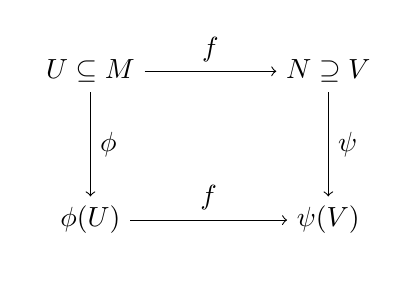
\begin{tikzpicture}
  \matrix (m) [matrix of math nodes, row sep=3.8em, column sep=4.8em, minimum width=2.2em]
  {
    U \subseteq M & N \supseteq V \\
    \phi(U) & \psi(V) \\
};
  \path[->]
  (m-1-1) edge node [above] {$f $} (m-1-2)
          edge node [auto] {$\phi$} (m-2-1)
  (m-1-2) edge node [auto]  {$\psi$} (m-2-2)
  (m-2-1) edge node [auto] {$f$} (m-2-2)
  ;
\end{tikzpicture}  
\quad \quad \, \begin{aligned} & \phi(p) = x \\
  & \psi(q) = y \end{aligned}
\]
$D(\psi f\varphi^{-1}) \equiv Df$.  $Df(p)$ injective (given $f$ immersion).  $Df(p) \in \text{Mat}(n,m)$

By change of basis in $\mathbb{R}^n$, assume $Df(p) = \left( \begin{matrix} I_m \\ 0 \end{matrix} \right)$.  

Now define $\begin{aligned} & \quad \\
  & G : \phi(U) \times \mathbb{R}^{n-m} \to \mathbb{R}^n \\
  & G(x,z) = f(x) + (0,z) \end{aligned}$

Thus, $DG(x,z) =1$ and for open $\phi(U) \times U_2$, $ G(\phi(U)\times U_2)$ open.  

By inverse function theorem, $G$ local diffeomorphism of $\mathbb{R}^n$, at $0$.  

Now $f = G\circ \mathfrak{i}$, where $\mathfrak{i}$ is canonical immersion.  
\[
\begin{gathered}
  G(x,0) = f(x) \\
  \Longrightarrow G^{-1}G(x,0) = (x,0) = G^{-1}f(x)
\end{gathered}
\]

Use $\psi \circ G$ as the local parametrization of $N$ around pt. $q$.  Shrink $U,V$ so that 

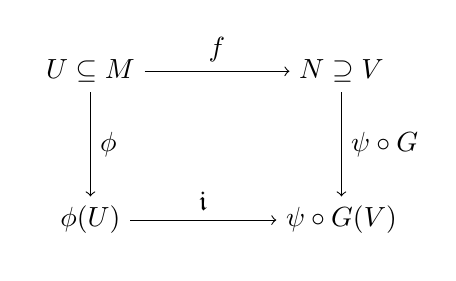
\begin{tikzpicture}
  \matrix (m) [matrix of math nodes, row sep=3.8em, column sep=4.8em, minimum width=2.2em]
  {
    U \subseteq M & N \supseteq V \\
    \phi(U) & \psi\circ G(V) \\
};
  \path[->]
  (m-1-1) edge node [above] {$f $} (m-1-2)
          edge node [auto] {$\phi$} (m-2-1)
  (m-1-2) edge node [auto]  {$\psi\circ G$} (m-2-2)
  (m-2-1) edge node [auto] {$\mathfrak{i}$} (m-2-2)
  ;
\end{tikzpicture}  

\end{proof}






\begin{theorem}[(Implicit Function Thm.)]
  Let open subset $U\subseteq \mathbb{R}^n \times \mathbb{R}^d$, $(x,y) = (x^1 \dots x^n, y^1 \dots y^k) $ on $U$.  \\
  Suppose smooth $\Phi:U\to \mathbb{R}^k$, $(a,b) \in U$, $c=\Phi(a,b)$

  If $k\times k$ matrix $\frac{ \partial \Phi^i}{ \partial y^j}(a,b)$ nonsingular, then $\exists $ neighborhoods $\begin{aligned} & \quad \\
    & V_0 \subseteq \mathbb{R}^n \text{ of $a$ } \\
    & W_0 \subseteq \mathbb{R}^k \text{ of $b$ } \end{aligned}$ and smooth $F:V_0 \to W_0$ s.t.

  $\Phi^{-1}(c) \bigcap (V_0\times W_0)$ is graph of $F$, i.e. \\
  $\Phi(x,y) =c$ for $(x,y) \in V_0\times W_0$ iff $y=F(x)$.  
  \end{theorem}



\subsection{Submersions} 
cf. pp. 20, Sec. 4 "Submersions", Ch. 1 of Guillemin and Pollack (2010) \cite{VGuilleminAPollack2010}.  

Consider $X,Y\in \text{\textbf{Man}}$, s.t. $\text{dim}X \geq \text{dim}Y$.  

\begin{definition}[submersion] If $f:X\to Y$, \\
if $Df_x \equiv df_x$ is \emph{surjective}, $f\equiv $ \textbf{submersion} at $x$.
\end{definition}
Recall that,  
\[
\begin{gathered}
	Df_x:T_xX \to T_{f(x)}Y \\
	\text{dim}T_xX \geq \text{dim}T_{f(x)}Y
\end{gathered}
\]
\[
\begin{gathered}
\text{rank}Df_x \leq \text{dim}T_{f(x)}Y, \text{ in general, while } \\
\text{rank}Df_x = \text{dim}T_{f(x)}Y \text{ iff } Df_x \text{ surjective }
\end{gathered}
\]

Canonical submersion is standard projection: \\
If $\begin{gathered} \quad \\
\text{dim}X = k \\
\text{dim}Y = l \end{gathered}$, $k\geq l$, 
\[
(a_1 \dots a_k ) \mapsto (a_1 \dots a_l)
\]

\begin{theorem}[Local Submersion Theorem]
	Suppose $f:X\to Y$ submersion at $x$, and $y = f(x)$, 
	Then $\exists \, $ local coordinates around $x$, $y$ s.t. 
	\[
	f(x_1\dots x_k) = (x_1 \dots x_l)
	\]
	i.e. $f$ locally equivalent to canonical submersion near $x$
\end{theorem}
\begin{proof}
I'll have a side-by-side comparison of my notation and the 1 used in Guillemin and Pollack (2010) \cite{VGuilleminAPollack2010} where I can.	

For charts $(U,\phi), (V,\psi)$ for $X,Y$, respectively, $y=f(x)$ for $x\in X$, 
\[
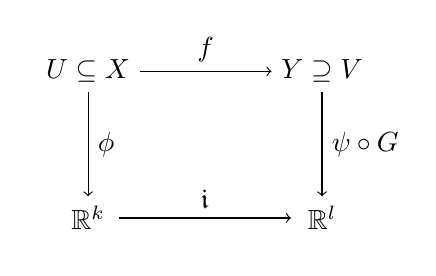
\begin{tikzpicture}
\matrix (m) [matrix of math nodes, row sep=3.8em, column sep=4.8em, minimum width=2.2em]
{
	U \subseteq X & Y \supseteq V \\
	\mathbb{R}^k &  \mathbb{R}^l \\
};
\path[->]
(m-1-1) edge node [above] {$f $} (m-1-2)
edge node [auto] {$\phi$} (m-2-1)
(m-1-2) edge node [auto]  {$\psi\circ G$} (m-2-2)
(m-2-1) edge node [auto] {$\mathfrak{i}$} (m-2-2)
;
\end{tikzpicture} \quad \quad \, 
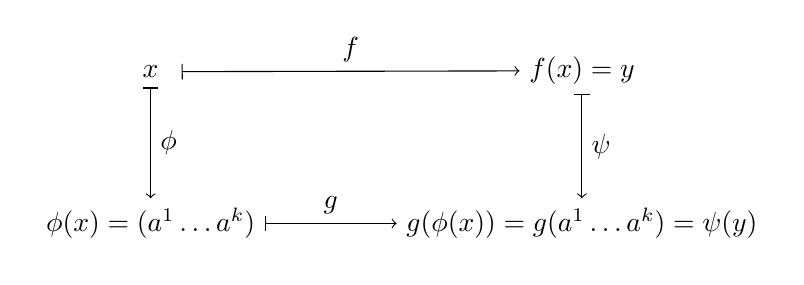
\begin{tikzpicture}
\matrix (m) [matrix of math nodes, row sep=3.8em, column sep=4.8em, minimum width=2.2em]
{
	 x & f(x)=y \\
	\phi(x)=(a^1\dots a^k) &  g(\phi(x))=g(a^1\dots a^k)=\psi(y) \\
};
\path[|->]
(m-1-1) edge node [above] {$f $} (m-1-2)
edge node [auto] {$\phi$} (m-2-1)
(m-1-2) edge node [auto]  {$\psi$} (m-2-2)
(m-2-1) edge node [auto] {$g$} (m-2-2)
;
\end{tikzpicture}
\]
$Dg_x$ surjective, so assume it's a $l\times k$ matrix $\left[ \begin{matrix} \mathbf{1}_l & 0 \end{matrix} \right]$.  

Define
\begin{equation}
\begin{aligned}
& G:U \subset \mathbb{R}^k \to \mathbb{R}^k  \\
& G(a)\equiv G(a^1\dots a^k) := (g(a), a_{l+1}, \dots , a_k)
\end{aligned}
\end{equation}
Now
\begin{equation}
DG(a)  = \left[ \begin{matrix} \mathbf{1}_l & 0 \\ & \mathbf{1}_{k-l} \end{matrix} \right] = \mathbf{1}_k
\end{equation}
so $G$ local diffeomorphism (at $0$).  

So $\exists \, $ $G^{-1}$ as local diffeomorphism of some $U'$ of $a$ into $U\subset \mathbb{R}^k$.  

By construction, 
\begin{equation}
g=\mathbb{P}_l \circ G
\end{equation}
where $\mathbb{P}_l$ is the \emph{canonical submersion}, the projection operator onto $\mathbb{R}^l$.  
\[
g\circ G^{-1} = \mathbb{P}_l
\]
(since $G$ diffeomorphism)

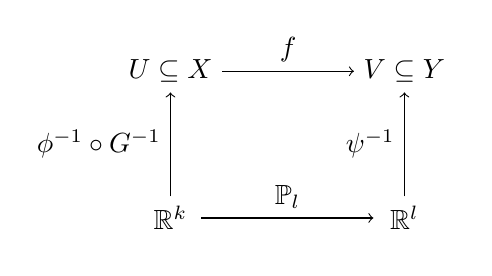
\begin{tikzpicture}
\matrix (m) [matrix of math nodes, row sep=3.8em, column sep=4.8em, minimum width=2.2em]
{
	U\subseteq X &  V\subseteq Y \\
	\mathbb{R}^k &  \mathbb{R}^l \\
};
\path[->]
(m-2-1) edge node [auto] {$\phi^{-1}\circ G^{-1}  $} (m-1-1)
edge node [auto] {$\mathbb{P}_l$} (m-2-2)
(m-1-1) edge node [auto]  {$f$} (m-1-2)
(m-2-2) edge node [auto] {$\psi^{-1}$} (m-1-2)
;
\end{tikzpicture}
for \\
$\Longrightarrow $ 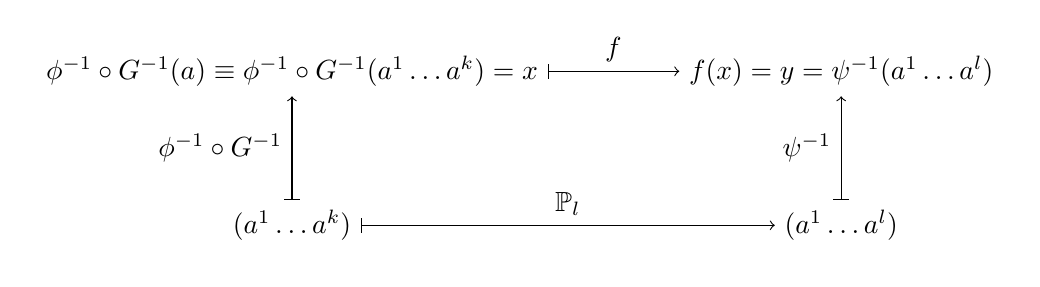
\begin{tikzpicture}
\matrix (m) [matrix of math nodes, row sep=3.8em, column sep=4.8em, minimum width=2.2em]
{
	\phi^{-1}\circ G^{-1}(a)\equiv \phi^{-1}\circ G^{-1}(a^1\dots a^k)=x & f(x)=y=\psi^{-1}(a^1\dots a^l) \\
	(a^1\dots a^k) &  (a^1\dots a^l) \\
};
\path[|->]
(m-2-1) edge node [auto] {$\phi^{-1}\circ G^{-1}  $} (m-1-1)
edge node [auto] {$\mathbb{P}_l$} (m-2-2)
(m-1-1) edge node [auto]  {$f$} (m-1-2)
(m-2-2) edge node [auto] {$\psi^{-1}$} (m-1-2)
;
\end{tikzpicture}


	\end{proof}
"An obvious corollary worth noting is that if $f$ is a submersion at $x$, then it is actually a submersion in a whole neighborhood of $x$." Guillemin and Pollack (2010) \cite{VGuilleminAPollack2010}

Suppose $f$ submersion at $x\in f^{-1}(y)$.  

By local submersion theorem
\[
f(x_1\dots x_k)=(x_1 \dots x_l)
\]
Choose $y=(0, \dots , 0)$. 

Then, near $x$, $f^{-1}(y) = \lbrace (0, \dots 0 , x_{l+1} \dots x_k)\rbrace$ i.e. let $V\ni x$ neighborhood of $x$, define $(x_1 \dots x_k)$ on $V$.  

Then $f^{-1}(y) \bigcap V = \lbrace (0\dots 0 , x_{l+1} , \dots x_k) | x_1 = 0 , \dots x_l = 0\rbrace$.

Thus $x_{l+1}, \dots x_k$ form a coordinate system on open set $f^{-1}(y) \bigcap V \subseteq f^{-1}(y)$.  

Indeed, 
\[
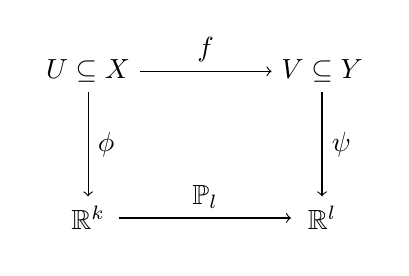
\begin{tikzpicture}
\matrix (m) [matrix of math nodes, row sep=3.8em, column sep=4.8em, minimum width=2.2em]
{
	U \subseteq X &  V\subseteq Y \\
	\mathbb{R}^k &  \mathbb{R}^l \\
};
\path[->]
(m-1-1) edge node [auto] {$ f  $} (m-1-2)
edge node [auto] {$ \phi $} (m-2-1)
(m-2-1) edge node [auto]  {$\mathbb{P}_l$} (m-2-2)
(m-1-2) edge node [auto] {$\psi$} (m-2-2)
;
\end{tikzpicture} \qquad \, 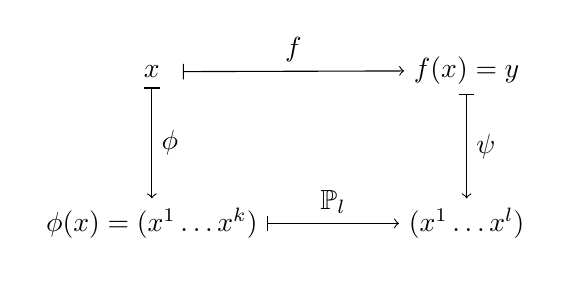
\begin{tikzpicture}
\matrix (m) [matrix of math nodes, row sep=3.8em, column sep=4.8em, minimum width=2.2em]
{
	x &  f(x)=y \\
	\phi(x)=(x^1\dots x^k) &  (x^1\dots x^l) \\
};
\path[|->]
(m-1-1) edge node [auto] {$ f  $} (m-1-2)
edge node [auto] {$ \phi $} (m-2-1)
(m-2-1) edge node [auto]  {$\mathbb{P}_l$} (m-2-2)
(m-1-2) edge node [auto] {$\psi$} (m-2-2)
;
\end{tikzpicture} 
\]
and now 
\[
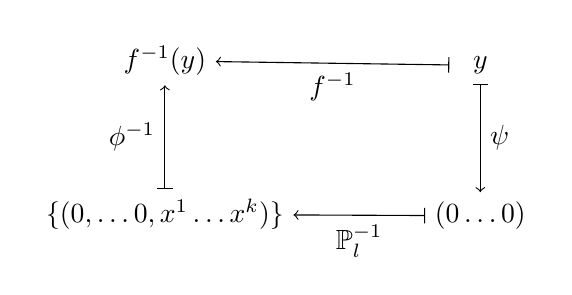
\begin{tikzpicture}
\matrix (m) [matrix of math nodes, row sep=3.8em, column sep=4.8em, minimum width=2.2em]
{
	f^{-1}(y) &  y \\
	\lbrace (0, \dots 0,x^1\dots x^k) \rbrace &  (0\dots 0) \\
};
\path[|->]
(m-1-2) edge node [auto] {$ f^{-1}  $} (m-1-1)
edge node [auto] {$ \psi $} (m-2-2)
(m-2-2) edge node [auto]  {$\mathbb{P}_l^{-1}$} (m-2-1)
(m-2-1) edge node [auto] {$\phi^{-1}$} (m-1-1)
;
\end{tikzpicture} 
\]

\begin{definition}[regular value]
	For smooth $f:X\to Y$, $X,Y \in \text{\textbf{Man}}$, \\
	$y\in Y$ is a \textbf{regular value} for $f$ if $Df_x:T_xX \to T_y Y$ surjective $\forall \, x$ s.t. $f(x)=y$.  
	
	$y\in Y$ \textbf{critical value} if $y$ not a regular value of $f$.  
\end{definition}



\begin{theorem}[Preimage theorem]
If $y$ regular value of $f:X\to Y$, \\
$f^{-1}(y)$ is a submanifold of $X$, with $\text{dim}f^{-1}(y)=\text{dim}X - \text{dim}Y$
\end{theorem}
\begin{proof}
Given $y$ is a regular value of $f:X\to Y$,  \\
$\forall \, x \in f^{-1}(y)$, $Df_x:T_xX \to T_yY$ is surjective.  By local submersion theorem, 
\[
f(x^1 \dots x^k) = (x^1 \dots x^l)=y
\]	
Since $x\in f^{-1}(y)$, $(x^1\dots x^k)=(y^1 \dots y^l,x^{l+1}\dots x^k)$.  

For this chart for $(U,\varphi)$, $U\ni x$, consider $(U\cap f^{-1}(y),\psi)$ with $\psi(x) = (x^{l+1}\dots x^k) \quad \, \forall \, x\in U\cap f^{-1}(y)$.  

$\forall \, f^{-1}(y)$ submanifold with $\text{dim}f^{-1}(y) = k-l = \text{dim}X-\text{dim}Y$.  
	\end{proof}

\emph{Examples for emphasis}

If $\text{dim}X > \text{dim}Y$, \\
\phantom{\qquad \, } if $y\in Y$, regular value of $f:X\to Y$, \\
\phantom{\qquad \, \qquad \, } $f$ submersion, $\forall \, x \in f^{-1}(y)$ \\
If $\text{dim}X = \text{dim}Y$, \\
\phantom{\qquad \, } $f$ local diffeomorphism $\forall \, x\in f^{-1}(y)$ \\
If $\text{dim}X < \text{dim}Y$, $\forall \, y\in f(X)$ is a critical value.  


\textbf{Example: $O(n)$ as a submanifold of $\text{Mat}(n,n)$}

Given $\text{Mat}(n,n)\equiv M(n) = \lbrace n \times n \text{ matrices } \rbrace$ is a manifold; in fact $\text{Mat}(n,n) \cong \mathbb{R}^{n^2}$, \\
Consider $O(n) = \lbrace A \in \text{Mat}(n,n) | AA^T = 1\rbrace$.  
\begin{equation}
AA^T \in \text{Sym}(n) \equiv S(n) = \lbrace S\in \text{Mat}(n,n) | S^T = S \rbrace = \lbrace \text{ symmetric $n\times n$ matrices } \rbrace
\end{equation}
$\text{Sym}(n)$ submanifold of $\text{Mat}(n,n)$, $\text{Sym}(n)$ diffeomorphic to $\mathbb{R}^k$ (i.e. $\text{Sym}(n) \cong \mathbb{R}^k$), $k:= \frac{n (n+1)}{2}$.  

\[
\begin{aligned}
	& f:\text{Mat}(n,n) \to \text{Sym}(n) \\
	& f(A) = AA^T
\end{aligned}
\]
Notice $f$ is smooth, 
\[
\begin{gathered}
f^{-1}(1) = O(n) \\
Df_A(B) = \lim_{s\to 0} \frac{ f(A+sB) - f(A) }{s} = \lim_{s\to 0} \frac{(A+sB)(A^T + sB^T)- AA^T}{s} = AB^T +BA^T
\end{gathered}
\]
If $Df_A : T_A\text{Mat}(n,n) \to T_{f(A)}\text{Sym}(n)$ surjective when $A\in f^{-1}(1) = O(n)$ (???).  





\begin{proposition} If smooth $g_1\dots g_l \in C^{\infty}(X)$ on $X$ are independent $\forall \, x\in X$, s.t. $g_i(x)=0$, $\forall \, i = 1\dots l$, \\
	then $Z=\lbrace x\in X | g_1(x) = \dots = g_l(x)=0 \rbrace = $ set of "common zeros" is a \emph{submanifold} of $X$ s.t. $\text{dim}Z = \text{dim}X- l$.  
	
	Take \emph{note} that $g_1 \dots g_l$ are independent at $x$ means, really, that $D(g_1)_x \dots D(g_l)_x$ are linearly independent on $T_xX$.  
\end{proposition}
\begin{proof}
Suppose smooth $g_1 \dots g_l \in C^{\infty}(X)$ on manifold $X$ s.t. $\text{dim}X = k\geq l$.  

Consider $g=(g_1\dots g_l):X \to \mathbb{R}^l$, $Z\equiv g^{-1}(0)$.  

Since $\forall \, g_i$ smooth, $D(g_i)_x:T_xX \to \mathbb{R}$ linear.  

Now for 
\[
Dg_x = (D(g_1)_x \dots D(g_l)_x):T_xX \to \mathbb{R}^l
\]	
By rank-nullity theorem (linear algebra), $Dg_x$ surjective iff $\text{rank}Dg_x = l$ i.e. $l$ functionals $D(g_1)_x \dots D(g_l)_x$ are linearly independent on $T_xX$.  

"We express this condition by saying the $l$ functions $g_1\dots g_l$ are independent at $x$."  (Guillemin and Pollack (2010) \cite{VGuilleminAPollack2010})  
	
	
	\end{proof}




Jeffrey Lee (2009) \cite{JLee2009}



John Lee (2012) \cite{JLee2012}


\section{Tensors}

I'll go through Ch.7 \emph{Tensors} of Jeffrey Lee (2009) \cite{JLee2009}.  

\begin{definition}[7.1\cite{JLee2009}] Let $V,W$ be modules over commutative ring $R$, with unity.  

Then, algebraic $W$-valued tensor on $V$ is multilinear map.  
\begin{equation}
	\tau: V_1 \times V_2 \times \dots \times V_m \to W
\end{equation}
where $V_i = \lbrace V,V^* \rbrace$ \quad \, $ \forall \, i=1,2,\dots m$.  

If for $r,s$ s.t. $r+s =m$, there are $r$ \, $V_i = V^*$, $s \, V_i = V$, tensor is $r$-contravariant, $s$-covariant; also say tensor of total type $\binom{r}{s}$.  
\end{definition}

EY : 20170404 Note that 
\[
\begin{aligned}
	& ( \tau_{\beta}^{i\alpha} \frac{ \partial }{ \partial x^i } \text{ or } \tau_{\beta}^{i\alpha} e_i )(\omega_j dx^j \text{ or } \omega_je^j  \in V^*) \\ 
	& ( \tau^{\beta}_{i\alpha} dx^i \text{ or } \tau^{\beta}_{i\alpha} e^i )( X^j \frac{ \partial }{ \partial x^j} \text{ or } X^j e_j  \in V) 
\end{aligned}
\]

$\exists \,$ natural map $\begin{aligned} & \quad \\ 
	& V\to V^{**} \\ 
& v \mapsto \widetilde{v} \end{aligned}$,  $\begin{aligned} & \quad \\ 
	& \widetilde{v} : \alpha \mapsto \alpha(v) \end{aligned}$.  If this map is an isomorphism, $V$ is \textbf{reflexive} module, and identify $V$ with $V^{**}$.  

\exercisehead{7.5} Given vector bundle $\pi: E \to M$, open $U\subset M$, consider sections of $\pi$ on $U$, i.e. cont. $s:U\to E$, where $(\pi\circ s)(u)=u$, \, $\forall \, u \in U$.  

Consider $E^* \ni \omega =\omega_i e^i$.  

$\forall \, s\in \Gamma(E)$, $\omega(s) = \omega_i(s(x))^i$, \, $\forall \, x \in U\subset M$.  So define $\widetilde{s}: \omega,x\mapsto \omega(s(x))$, \, $\forall \, x \in U$.  

If $\widetilde{s} =0$, $\widetilde{s}(\omega,x) = \omega(s(x)) =0$ \quad \, $\forall \, \omega \in E^*$, $\forall \, x\in U$, and so $s=0$.  (Let $\omega_i = \delta_{iJ}$ for some $J$, and so $s^J(x) =0$ \quad \, $\forall \, J$).  

$s=0$.  So $\text{ker}(s\mapsto \widetilde{s}) = \lbrace 0 \rbrace$ (so condition for injectivity is fulfilled).  

Since $\widetilde{s}:\omega,x\mapsto \omega(s(x))$, $\forall \, \omega \in E^*$, $\forall \, x \in U$, $s\mapsto \widetilde{s}$ is surjective.  

$s\mapsto \widetilde{s}$ is an isomorphism so $\Gamma(E)$ is a \emph{reflexive} module.  


\begin{proposition}
For $R$ a ring (special case), $\exists \, $ module homomorphism:  \\

tensor product space $\to $ tensor, as a multilinear map, i.e. $\exists$ \,  
\begin{equation}
\begin{aligned}
&	\left( \otimes_{i=1}^r V \right) \otimes \left( \otimes_{j=1}^s V^* \right) \to T^r_{ \, \, s}(V;R)   \\
& u_1 \otimes \dots \otimes u_r \otimes \beta^1 \otimes \dots \otimes \beta^s \in \left( \otimes^r V \right) \otimes \left( \otimes^s V^* \right) \mapsto (\alpha^1 \dots \alpha^r, v_1 \dots v_s) \mapsto \alpha^1(u_1) \dots \alpha^r(u_r) \beta^1(v_1) \dots \beta^s(v_s)  
\end{aligned}
\end{equation}
\end{proposition}

Indeed, consider 
\[
(\alpha^1 \dots \alpha^r, v_1 \dots v_s) \in \underbrace{V^* \times \dots \times V^* }_{r} \times \underbrace{ V\times \dots \times V}_{s} \mapsto \alpha^1(u_1) \dots \alpha^r(u_r) \beta^1(v_1) \dots \beta^s(v_s)
\]
and so for 
\[
\begin{aligned}
	& \alpha^i = \alpha^i_{\mu} e^{\mu} , \, & \, i =1,2, \dots r, \, & \, \mu = 1,2, \dots \text{dim}V^* \\ 
	& v_i = v_i^{\mu} e_{\mu} , \, & \, i = 1,2, \dots s, \, & \, \mu = 1, 2, \dots \text{dim}V 
\end{aligned} \qquad \, \begin{aligned}
& \alpha^i(u_i) = \alpha^i_{\mu} u^{\mu}_i \\ 
 & \beta^i(v_i) = \beta^i_{\mu} v^{\mu}_i
\end{aligned}
\]
So that 
\[
\begin{gathered}
	\alpha^1(u_1) \dots \alpha^r(u_r) \beta^1(v_1) \dots \beta^s(v_s) = \alpha^1_{\alpha_1}u^{\alpha_1}_1 \dots \alpha^r_{\alpha_r} u^{\alpha_r}_r \beta^1_{\mu_1} v^{\mu_1}_1 \dots \beta^s_{\mu_s} v^{\mu_s}_s = \\
	= (u^{\alpha_1}_1 \dots u_r^{\alpha_r} \beta^1_{\mu_1} \dots \beta^s_{\mu_s})(\alpha^1_{\alpha_1} \dots \alpha^r_{\alpha_r} v_1^{\mu_1} \dots v_s^{\mu_s} )
\end{gathered}
\]
Identify $u_1 \otimes \dots \otimes u_r \otimes \beta^1 \otimes \dots \otimes \beta^s$ with this multiplinear map.  

\begin{proposition}
If $V$ is finite-dim. vector space, or if $V=\Gamma(E)$, for vector bundle $E\to M$, map
\begin{equation}
\left( \otimes_{i=1}^r V \right)  \otimes \left( \otimes_{j=1}^s V^* \right) \to T^r_{ \, \, s}(V;R)
\end{equation}
is an isomorphism.  
\end{proposition}

\begin{definition}
tensor that can be written as 
\begin{equation}
u_1\otimes \dots \otimes u_r \otimes \beta^1 \otimes \dots \otimes \beta^s \equiv u_1\otimes \dots \otimes \beta^s 
\end{equation}
is \textbf{simple} or \textbf{decomposable}.  
\end{definition}
Now well that not \emph{all} tensors are simple.  

\begin{definition}[7.7\cite{JLee2009}, tensor product]
$\forall \, S\in T^{r_1}_{ \,\, s_1}(V)$, $\forall \, T \in T^{r_2}_{ \,\, s_2}(V)$, \\
define tensor product 
\begin{equation}
\begin{gathered}
S\otimes T\in T^{r_1+r_2}_{ \, \, \, s_1+s_2}(V) \\
	S\otimes T( \theta^1\dots \theta^{r_1 + r_2}, v_1 \dots v_{s_1+s_2}) := S(\theta^1\dots \theta^{r_1}, v_1\dots v_{s_1})T(\theta^{r_1+1}\dots \theta^{r_1+r_2}, v_{s_1+1}\dots v_{s_1 + s_2} )
\end{gathered}
\end{equation}
\end{definition}

\begin{proposition}[7.8\cite{JLee2009}]
\end{proposition}







\[
\begin{gathered}
	\tau^{ i_1 \dots i_r }_{ \phantom{i_1 \dots i_r} j_1 \dots j_s} e_{i_1} \otimes \dots \otimes e_{i_r} \otimes e^{j_1}\otimes \dots \otimes e^{j_s} = \tau(e^{i_1} \dots e^{i_r}, e_{j_1} \dots e_{j_s} )e_{i_1} \otimes \dots \otimes e_{i_r} \otimes e^{j_1} \otimes \dots \otimes e^{j_s} = \tau 
\end{gathered}
\]
So $\lbrace e_{i_1}\otimes \dots \otimes e_{i_r} \otimes e^{j_1} \otimes \dots \otimes e^{j_s} | i_1 \dots i_{r}, j_1\dots j_s \in 1 \dots n \rbrace$ spans $T^r_{\,\, s}(V;R)$

\exercisehead{7.11}  Let basis for $V$ \, $e_1 \dots e_n$, corresponding dual basis for $V^*$ \,  $e^1 \dots e^n$ \\ 
Let basis for $V$ \, $\overline{e}_1 \dots \overline{e}_n$, corresponding dual basis for $V^*$ \,  $\overline{e}^1 \dots \overline{e}^n$ \\
s.t. 
\[
\begin{aligned}
	& \overline{e}_i = C^k_{ \,\, i} e_k \\
	& \overline{e}^i = (C^{-1})^i_{ \, \, k} e^k
\end{aligned}
\]
EY:20170404, keep in mind that
 
\[
\begin{aligned}
	&	Ax = e_i A^i_{ \, \, k} e^k(x^j e_j) = e_i A^i_{ \,\,j} x^j = A^i_{ \, \, j} x^j e_i \\ 
 & Ae_j = e_k A^k_{ \, \, i} e^i (e_j) = A^k_{ \,\, j} e_k = \overline{e}_j
\end{aligned}
\]
\[
\begin{gathered}
\overline{\tau}^i_{ \,\, jk} \overline{e}_i \otimes \overline{e}^j \otimes \overline{e}^k = \overline{\tau}^i_{ \, \, jk} C^l_{ \, \, i} e_l (C^{-1})^j_{ \,\, m} e^m(C^{-1})^k_{ \, \, n} e^n = \overline{\tau}^i_{ \, \, jk} C^l_{ \, \, i } (C^{-1})^j_{ \,\, m} (C^{-1})^k_{ \,\, n} = \tau^l_{ \,\, mn}   \\
\overline{\tau}^i_{ \,\, jk} = C^c_{ \,\, k} C^b_{ \,\, j} (C^{-1})^i_{ \,\, a} \tau^a_{\,\, bc}
\end{gathered}
\]



On Remark 7.13 of Jeffrey Lee (2009) \cite{JLee2009}:  first, egregious typo for $L(V,V)$; it shoudl be $L(V,W)$.  Onward, \\
for $L(V,W)$, \\
consider $W\otimes V^* \ni w\otimes \alpha$ s.t.
\[
(w\otimes \alpha)(v) = \alpha(v)w\in W, \, \forall \, v\in V, \text{ so } w\otimes \alpha \in L(V,W)
\]

Now consider (category of) left $R$-module, 
\begin{equation}
{\,}_R\textbf{Mod} \ni {\,}_{\text{Mat}_{\mathbb{K}}(N,M) } \mathbb{K}^N
\end{equation}
where
\[
\begin{aligned}
	& V=\mathbb{K}^N \\ 
&	  W = \mathbb{K}^M
\end{aligned}
\]
For $A\in \text{Mat}_{\mathbb{K}}(N,M)$, $x\in \mathbb{K}^N$, 
\[
e_i A^i_{ \,\ , \mu} e^{\mu}(x^{\nu} e_{\nu}) = Ax = e_iA^i_{\,\, \mu} x^{\mu} , \quad \, i=1,2,\dots M, \, \mu = 1,2, \dots N
\]
\[
A\in \text{Mat}_{\mathbb{K}}(N,M) \cong W\otimes V^* \cong L(V,W)
\]
Consider 
\[
\begin{aligned}
	& \alpha \in (\mathbb{K}^N)^* = V^* \\
	& w\in \mathbb{K}^M = W
\end{aligned} \qquad \, \begin{aligned}
	& \alpha = \alpha_{\mu} e^{\mu} \\ 
	& w=w^ie_i
\end{aligned}
\]
\[
\alpha \otimes w = w \otimes \alpha = w^i\alpha_{\mu} e_i \otimes e^{\mu}
\]
(remember, isomoprhism between $\text{Mat}_{\mathbb{K}}(N,M)$ and $W\otimes V^*$ guaranteed, if $V,W$ are free $R$-modules, $R=\mathbb{K}$).

Let $V,W$ be left $R$-modules, i.e. $V,W \in {\,}_R\text{\textbf{Mod}}$.  
\[
V^* \in \text{\textbf{Mod}}_R
\]
For $V^*\otimes W \in \text{\textbf{Mod}}_R\otimes {\,}_R\text{\textbf{Mod}}$  
\[
\alpha \in V^*, w\in W
\]
\[
(\alpha \otimes w)(v) = \alpha(v)w, \text{ for } v\in V \in {\,}_R\text{\textbf{Mod}}
\]
But $(w\otimes \alpha)(v) = w\alpha(v)$.  

Note $\alpha(v) \in R$.  

Let $V,W$ be right $R$-modules, i.e. $V,W \in \text{\textbf{Mod}}_R$.  
\[
V^* \in {\,}_R\text{\textbf{Mod}}
\]
For $W\otimes V^* \in \text{\textbf{Mod}}_R \otimes {\,}_R\text{\textbf{Mod}}$.  
\[
\alpha \in V^*, \, w\in W
\]
\[
(v)(w\otimes \alpha) = w\alpha(v), \text{ with } \alpha(v)\in R, \, v\in V
\]
So $W\otimes V^* \cong L(V,W)$, for $V,W\in \text{\textbf{Mod}}_R$

\begin{definition}[7.20\cite{JLee2009}, \textbf{contraction}]
Let $(e_1,\dots e_n)$ basis for $V$, $(e^1\dots e^n)$ dual basis.  

If $\tau \in T^r_{ \,\, s}(V)$, then for $k\leq r$, $l\leq s$, define 
\begin{equation}
\begin{gathered}
	C^k_l \tau \in T^{r-1}_{ \, \, s-1}(V) \\ 
 C^k_l\tau(\theta^1 \dots \theta^{r-1}, w_1\dots w_{s-1}) := \\
	\sum_{a=1}^n \tau(\theta^1 \dots \underbrace{e^a}_{\text{$k$th position} } \dots \theta^{r-1}, w_1 \dots \underbrace{e_a}_{\text{$i$th position}} \dots w_{s-1}  )
\end{gathered}
\end{equation}
$C^k_l$ is called \textbf{contraction}, for some single $1\leq k \leq r$, some single $1\leq l \leq s$, 
\[
C^k_l: T^r_s(V) \to T^{r-1}_{s-1}(V)
\]
s.t.
\[
(C^k_l\tau)^{i_1\dots \widehat{i}_k\dots i_r }_{ \phantom{i_1\dots \widehat{i}_k\dots i_r} j_1\dots \widehat{j}_l \dots j_s} := \tau^{i_1\dots a \dots i_r}_{ \phantom{i_1\dots a \dots i_r} j_1 \dots a \dots j_s }
\]
\end{definition}

Universal mapping properties can be invoked to give a basis free definition of contraction (EY : 20170405???).  

IN general, 
\[
\forall \, v_1 \dots v_s \in V, \forall \, \alpha^1 \dots \alpha^r \in V^*
\]
so that 
\[
\begin{aligned}
	& v_j = v_j^{\mu} e_{\mu} \\ 
	& \alpha^i = \alpha^i_{\mu} e^{\mu}
\end{aligned} \quad \, \begin{aligned}
	& j=1\dots s, \quad \, \mu = 1,\dots \text{dim}V \\ 
	& i=1\dots r, \quad \, \mu = 1\dots \text{dim}V^*
\end{aligned}
\]
then $\forall \, \tau \in T^r_{ \,\, s} (V)$, 
\[
\begin{gathered}
	\tau(\alpha^1\dots \alpha^r,v_1\dots v_s) = \tau( \alpha^1_{\mu_1} e^{\mu_1} \dots \alpha^r_{\mu_r} e^{\mu_r} , v_1^{\nu_1} e_{\nu_1} \dots v_s^{\nu_s}e_{\nu_s} ) = \\ 
	= \alpha^1_{\mu_1} \dots \alpha^r_{\mu_r} v_1^{\nu_1} \dots v_s^{\nu_s} \tau(e^{\mu_1}\dots e^{\mu_r} , e_{\nu_1} \dots e_{\nu_s} ) = \alpha^1_{\mu_1} \dots  \alpha_{\mu_r}^r v_1^{\nu_1} \dots v_s^{\nu_s} \tau^{\mu_1 \dots \mu_r}_{ \phantom{\mu_1 \dots \mu_r} \nu_1\dots \nu_s}
\end{gathered}
\]
which is equivalent to
\[
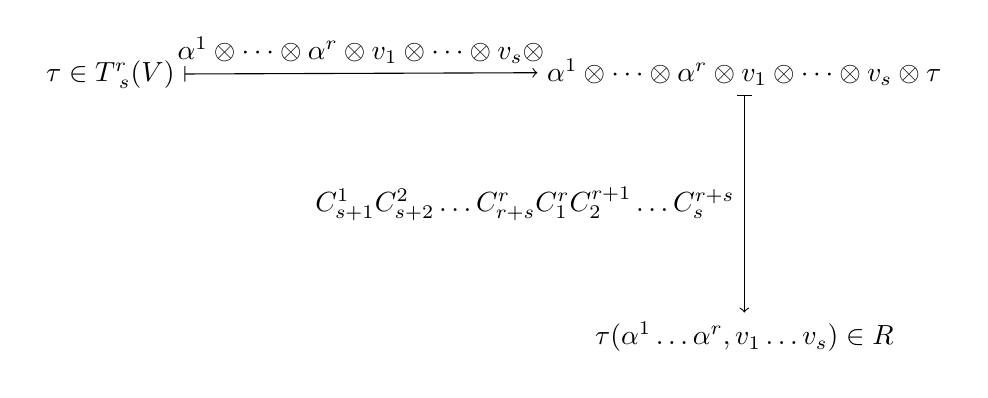
\begin{tikzpicture}
  \matrix (m) [matrix of math nodes, row sep=7.8em, column sep=12.8em, minimum width=5.2em]
  {
  \tau \in T^r_{\,\,s}(V)  &  \alpha^1 \otimes \dots \otimes \alpha^r \otimes v_1\otimes \dots \otimes v_s \otimes \tau  \\ 
& \tau(\alpha^1\dots \alpha^r,v_1\dots v_s)  \in R \\ 
};
  \path[|->]
  (m-1-1) edge node [above] {$ \alpha^1\otimes \dots \otimes \alpha^r \otimes v_1 \otimes \dots \otimes v_s \otimes $} (m-1-2)
  (m-1-2) edge node [left] {$C^1_{ s+1} C^2_{s+2}\dots C^r_{r+s} C^r_1 C_2^{r+1}\dots C_s^{r+s} $} (m-2-2)
  ;
\end{tikzpicture}  
\]
where I've tried to express the right-$R$-module, "right action" on $\alpha^1 \otimes \dots \otimes \alpha^r \otimes v_1\otimes \dots \otimes v_s \in V^*\otimes \dots \otimes V$.  


Conlon (2008) \cite{Conl2008}


\part{Pr\'{a}staro}

Pr\'{a}staro (1996) \cite{Pras1996}

\subsubsection{Affine Spaces}

cf. Sec. 1.2 - \emph{Affine Spaces} of Pr\'{a}staro (1996) \cite{Pras1996}

\begin{definition}[affine space]
  \begin{equation}
\begin{gathered}
    \text{ affine space \qquad \, } (M, \mathbf{M}, \alpha )  \\
    \text{ with } \\
    \begin{aligned}
      & M \equiv \text{ set (set of pts.) }  \\ 
      & \mathbf{M} \equiv \text{ vector space (space of free vectors) } \\
      & \alpha \equiv \mathbf{M} \times M \to M \equiv \text{ translation operator } \\
      & \alpha : (v,p ) \mapsto p' \equiv p + v
      \end{aligned}
\end{gathered}
  \end{equation}
  Note: $\alpha$ is a \textbf{transitive} action and without fixed pts. (free).

  i.e. $\forall \, p \in M$, 
  \end{definition}

$\forall \, $ pt. $O \in M$, $\alpha:(v,O) \mapsto O' \equiv O + v$, $\alpha (\cdot , O) \equiv \alpha_O \equiv \alpha(O)$.  $\alpha_O(v) = O' = O + \mathbf{v}$ \qquad \, $\forall \, O' \in M$, $\exists \, \mathbf{v} \in \mathbf{M}$ s.t. $O' = O + \mathbf{v}$ \\
$\Longrightarrow M \equiv \mathbf{M}$.

$\forall \, (O, \lbrace e_i \rbrace)_{1 \leq i \leq n }$, where $\lbrace e_i \rbrace$ basis of $\mathbf{M}$, $M \equiv \mathbf{M} = \mathbb{R}^n$ so isomorphism $M \simeq \mathbb{R}^n$ \\
\begin{definition}
  $(O, \lbrace e_i \rbrace) \equiv $ affine frame.

  $\forall \, $ affine frame $(O,\lbrace e_i \rbrace)$, $\exists \, $ coordinate system $x^{\alpha} : M \to \mathbb{R}$, \\
  where $x^{\alpha}(p)$ is $\alpha$th component, in basis $\lbrace e_i \rbrace$, of vector $p-O$
  \end{definition}

\begin{theorem}[1.4 Pr\'{a}staro (1996) \cite{Pras1996}]
  Let $(x^{\alpha}), (\overline{a}^{\alpha})$ 2 coordinate systems correspond to affine frames $(O, \lbrace e_i \rbrace)$, $( \overline{O}, \lbrace \overline{e}_i \rbrace )$, respectively.
\begin{equation}
  \overline{x}^{\alpha} = A^{\alpha}_{ \, \, \beta} x^{\beta} + y^{\alpha}
\end{equation}
where
\[
y^{\alpha} \in \mathbb{R}^n, \qquad \, A^{\alpha}_{ \, \, \beta} \in GL(n; \mathbb{R})
\]
\end{theorem}

\begin{definition}[1.10 Pr\'{a}staro (1996) \cite{Pras1996}]
  \begin{equation}
    A(n) \equiv Gl(n,\mathbb{R}) \times \mathbb{R}^n
  \end{equation}
  affine group of dim. $n$
  \end{definition}

\begin{theorem}[1.5] symmetry group of $n$-dim. affine space, called affine group $A(M)$ of $M$.  $\exists \, $ isomoprhism,
  \begin{equation}
    A(M) \simeq A(n), \qquad \, f\mapsto (f^{\alpha}_{ \, \, \beta} , y^{\alpha}) \, ; \qquad \, f^{\alpha} \equiv x^{\alpha} \circ f = f^{\alpha}_{ \, \, \beta} x^{\beta} + y^{\alpha}
  \end{equation}
cf. Eq. 1.4 Pr\'{a}staro (1996) \cite{Pras1996}
  \end{theorem}





\part{Holonomy}

\begin{definition}[Conlon, 10.1.2] If $X,Y\in \mathfrak{X}(M)$, $M\subset \mathbb{R}^m$, \textbf{Levi-Civita connection} on $M\subset \mathbb{R}^m$
	\begin{equation}
	\begin{aligned}
	& \nabla : \mathfrak{X}(M) : \mathfrak{X}(M) \to \mathfrak{X}(M) \\
	\nabla_XY := p(D_XY)
	\end{aligned}
	\end{equation}
	with 
	\[
	D_XY := \sum_{j=1}^m X(Y^j) \frac{ \partial }{ \partial x^j} = \sum_{i,j=1}^m X^i \frac{ \partial Y^j}{ \partial x^i} \frac{ \partial }{ \partial x^j} \qquad \,  \begin{aligned} & \quad \\ 
		& \forall \, X=\sum_{i=1}^m X^i \frac{ \partial }{ \partial x^i},  \\
		& \forall \, Y=\sum_{i=1}^m Y^i \frac{\partial }{ \partial x^i } \end{aligned}
	\]
\end{definition}

\[
\begin{aligned}
	& \nabla_{fX}Y = f(D_{fX}Y) = p(fD_XY) = fpD_XY = f\nabla_XY \\ 
	&  \nabla_X fY = p(D_XfY) = p \left( \sum_{i,j=1}^m \left( X^i f\frac{ \partial Y^j}{ dx^i } + X^i Y^j \frac{ \partial f}{ \partial x^i} \right) \frac{ \partial }{ \partial x^j} \right) = f\nabla_X Y + p \sum_{j=1}^m X(f) Y^j \frac{ \partial }{ \partial x^j} = f\nabla_XY + X(f) p(Y)
\end{aligned}
\]


\begin{definition}[Conlon, 10.1.4; Christoffel symbols] 
\begin{equation}
\begin{gathered}
	\nabla_{\frac{ \partial }{ \partial x^i} \frac{ \partial }{ \partial x^j} = \Gamma^k_{ij} \frac{ \partial }{ \partial x^k} \qquad \, \text{ (Conlon's notation) }  }   \\
	\nabla_{\frac{ \partial }{ \partial x^j} \frac{ \partial }{ \partial x^i} = \Gamma^k_{ij} \frac{ \partial }{ \partial x^k} \qquad \, \text{ (F. Schuller's notation) }  }
\end{gathered}
\end{equation}
\end{definition}





\begin{definition}[torsion]
\begin{equation}
\begin{aligned}
	& T:\mathfrak{X}(M) \in \mathfrak{X}(M) \to \mathfrak{X}(M) \\ 
	& T(X,Y) = \nabla_XY - \nabla_Y X - [X,Y] 
\end{aligned}
\end{equation}
If $T=0$, $\nabla$ torsion-free or symmetric.  
\end{definition}
\[
\begin{gathered}
T(fX,Y) = f\nabla_XY - (f\nabla_Y X + Y(f)X) - \lbrace (fXY - (Y(f)X + fYX) \rbrace = fT(X,Y) \\ 
T(X,fY) = f\nabla_XY + X(f)Y - f\nabla_Y X   - \lbrace ( ( X(f) Y +fXY) -  fYX \rbrace = fT(X,Y)  
\end{gathered}
\]
Thus, $T(X,Y)$ $C^{\infty}(M)$-bilinear.  

$T\in \tau_1^2 (M)$.  

$T(v,w) \in T_xM$ defined, $\forall \, v,w \in T_xM$, $\forall \, x\in M$.

Thus, torsion is a \textbf{tensor}.

\exercisehead{10.1.7 Conlon (2008)\cite{Conl2008} }.  

If $T(X,Y)=0$,
\[
T(e_i,e_j) = \Gamma^k_{ji} e_k - \Gamma^k_{ij} e_k - 0 = 0 \Longrightarrow \Gamma_{ji}^k = \Gamma^k_{ij}
\]

If $\Gamma^k_{ij} = \Gamma^k_{ji}$, $T(e_i,e_j)=0$.  

\exercisehead{10.1.8, Conlon (2008)\cite{Conl2008}} 

If $M\subset \mathbb{R}^m$ smoothly embedded submanifold,  
$\forall \, \frac{ \partial }{ \partial x^j}, \frac{ \partial }{ \partial x^i} \in T_xM$, spanning $T_xM$, consider $\frac{ \partial }{ \partial x^j} = X^k_j \frac{ \partial }{ \partial \widetilde{x}^k}$, $\frac{ \partial }{ \partial x^i} = X_i^k(\widetilde{x}) \frac{ \partial }{ \partial \widetilde{x}^k}$  

\[
\begin{gathered}
	\nabla_{\frac{\partial }{ \partial x^j} } \frac{ \partial }{ \partial x^i} = p D_{ X^k_j \frac{ \partial }{ \partial \widetilde{x}^k } } X^l_i \frac{ \partial }{ \partial \widetilde{x}^l } = p \left( X^k_j \frac{ \partial X^l_i}{  \partial \widetilde{x}^k } \frac{ \partial }{ \partial \widetilde{x}^l } \right) =   X^k_j  p \left( \frac{ \partial X^l_i}{  \partial \widetilde{x}^k } \frac{ \partial }{ \partial \widetilde{x}^l } \right)  \\ 
	\nabla_{\frac{\partial }{ \partial x^i} } \frac{ \partial }{ \partial x^j} =  X^k_i p \left(  \frac{ \partial X^l_j }{ \partial \widetilde{x}^k }   \frac{ \partial }{ \partial \widetilde{x}^l  } \right) 
\end{gathered}
\]









If $X\in \mathfrak{X}(M)$, smooth $s:[a,b]\to M$, 

then $\forall \, s(t)$, 
\[
X'_{s(t)} = \nabla_{\dot{s}(t)} X \in T_{s(t)}M
\]
In fact, it's often natural to consider fields $X_{s(t)}$ along $s$, parametrized by parameter $t$, allowing
\[
X_{s(t_1)} \neq X_{s(t_2)}
\]
each of $s(t_1)=s(t_2)$.  

\begin{definition}[10.1.9] Let smooth $s:[a,b] \to M$.  

Vector field along $s$ is smooth $v:[a,b]\to TM$ s.t. 
\[
\begin{tikzpicture}
  \matrix (m) [matrix of math nodes, row sep=7.8em, column sep=12.8em, minimum width=5.2em]
  {
   &  TM  \\ 
	\left[ a,b \right] & M \\ 
};
  \path[|->]
  (m-2-1) edge node [above] {$ v $} (m-1-2)
edge node [above] {$s$} (m-2-2)
  (m-1-2) edge node [left] {$ \pi $} (m-2-2)
  ;
\end{tikzpicture}  
\]
commutes.

Note that $v\in \mathfrak{X}(s) \subset \mathfrak{X}(M)$
\end{definition}

e.g. $(Y|s)(t) = Y_{s(t)}$, restriction of $Y\in \mathfrak{X}(M) $ to $s$.  

e.g. $\dot{s}(t) \in \mathfrak{X}(M)$.  

$\forall \, v,w \in \mathfrak{X}(s)$, $v+w \in \mathfrak{X}(s)$, 
\[
\begin{gathered}
	(fv+gv)(t) := (f(s(t)) + g(s(t)) )v(t) = f(s(t)) v(t) + g(s(t)) v(t) = (f+g)v(t)
\end{gathered}
\]
Likewise, 
\[
f(v+w) = fv+fw
\]
$\mathfrak{X}(s)$ is a real vector space and $C^{\infty}[a,b]$-module.  

\begin{definition}[10.1.10]
Let conection $\nabla$ on $M$.  

\textbf{Associated covariant derivative} is operator 
\[
\frac{\nabla}{dt} \mathfrak{X}(s) \to \mathfrak{X}(s)
\]
$\forall \, $ smooth $s$ on $M$, s.t. 
\begin{enumerate}
\item $\frac{\nabla}{dt}$ $\mathbb{R}$-linear 
\item $\left( \frac{\nabla}{dt} \right)(fv) = \frac{df}{dt} v+ f\frac{\nabla}{dt} v$, $\forall \, f \in C^{\infty}[a,b]$, $\forall \, v\in \mathfrak{X}(s)$  
\item If $Y\in \mathfrak{X}(M)$, then
\[
\frac{\nabla}{dt} (Y|s)(t) = \nabla_{ \dot{s}(t)}Y \in T_{s(t)} M, \quad \, a\leq t \leq b
\]
\end{enumerate}
\end{definition}












\begin{theorem}[Conlon Thm. 10.1.11\cite{Conl2008} ]
	$\forall \, $ connection $\nabla$ on $M$, $\exists \, !$ \, associated covariant derivative $\frac{ \nabla }{dt}$
\end{theorem}

\begin{proof}
	Consider arbitrary coordinate chart $(U,x^1 \dots x^n)$.  
	
	Consider smooth curve $s:[a,b]\to U$.  
	
	Let $v\in \mathfrak{X}(s)$, $v(t) = v^i(t) \frac{ \partial }{ \partial x^i}$; $\dot{s}(t) = s^j \frac{ \partial }{ \partial x^j}$.  
	\[
	\begin{gathered}
	\frac{ \nabla v}{ dt} = \frac{dv^i(t) }{dt}\frac{ \partial }{ \partial x^i} + v^i(t) \frac{ \nabla}{dt} \frac{ \partial }{ \partial x^i} = \frac{ d v^i }{dt}	\frac{ \partial }{ \partial x^i} + v^i \nabla_{ \dot{s}(t) } \frac{ \partial }{ \partial x^i } = \dot{v}^i \frac{ \partial }{ \partial x^i } + v^i\dot{s}^j \Gamma^k_{ij} \frac{ \partial }{ \partial x^k} = \left( \dot{v}^k + v^i \dot{s}^j \Gamma^k_{ij} \right)\frac{ \partial }{ \partial x^k} \end{gathered}
	\]
	This is an explicit, local formula in terms of connection, proving uniqueness.  
	
	Existence: $\forall \, $ coordinate chart $(U,x^1\dots x^n)$, $\left( \dot{v}^k + v^i \dot{s}^j \Gamma_{ij}^k \right) \frac{ \partial }{ \partial x^k } =: \frac{ \nabla v}{dt}$.  
	
	\[
	\begin{gathered}
	\frac{\nabla}{dt}(fv) = \dot{f}v^k + f\dot{v}^k + fv^i \dot{s}^j = \dot{f}v + f\frac{ \nabla v}{dt}
	\end{gathered}
	\]
If $f$ constant, then $\frac{\nabla}{dt}$ is $\mathbb{R}$-linear.  	

\end{proof}

\begin{definition}[10.1.12 Conlon (2008)\cite{Conl2008}]
	Let $(M,\nabla)$.  Let $v\in\mathfrak{X}(s)$ for smooth $s:[a,b] \to M$.  

If $\frac{\nabla v}{dt} \equiv 0$ on $s$, then $v$ is \textbf{parallel } along $s$.  
\end{definition}

\begin{theorem}[10.1.13] 
Let $(M,\nabla)$, smooth $s:[a,b]\to M$, $c\in [a,b]$, $v_0 \in T_{s(c)}M$.  

Then $\exists \, !$ parallel field $v\in \mathfrak{X}(s)$ s.t. $v(c) = v_0$.  

$v$ parallel transport along $s$.  
\end{theorem}
\begin{proof}
	\[
\begin{aligned}
	& \dot{s}(t) = \dot{s}^j(t) e_j \\ 
	&  v(t) = v^i(t) e_i  \\
& v_0 = a^i e_i
\end{aligned}
\]
\[
0 = \left( \frac{dv^k}{dt}(t) + v^i(t) \dot{s}^j(t) \Gamma^k_{ij}(s(t)) \right) e_k
\]
or equivalently
\begin{equation}
	\frac{dv^k}{dt} = - v^i \dot{s}^j \Gamma^k_{ij} , \qquad \, 1\leq k \leq n \qquad \, (10.1)
\end{equation}
with initial conditions $v^k(c) = a^k$, $1\leq k \leq n$.  

By existence and uniqueness of solutions of O.D.E.  

$\exists \, \epsilon > 0$ s.t. $\exists \, !$ solutions $v^k(t)$.  For $c-\epsilon < t < c+\epsilon$.  

In fact, these ODEs being linear in $v^k$,  by ODE theory (Appendix C, Thm. C.4.1).  

$\nexists \, $ restriction on $\epsilon$, so $\exists \, ! \, v^k(t)$ \, $\forall \, t \in [a,b]$, $1\leq k \leq n$  

\end{proof}




\subsubsection{Principal bundle, vector bundle case for parallel transport}  

Recall the 2 different forms or viewpoints for Lie-algebra valued 1-forms, or vector-valued 1-forms, or sections of 1-form-valued endomorphisms:
\[
\omega^k_{ \,\, i\mu} dx^{\mu} \equiv \omega^k_{\,\,i} \in \Omega^1(M,\mathfrak{gl}(n,\mathbb{F})) = \Gamma(\mathfrak{gl}(n,\mathbb{R} \otimes \left. T^* M \right|_U ) )
\] 
for $\begin{aligned} & \quad \\
	& i,k = 1\dots n =\text{dim}E \\ 
	& \mu = 1\dots d =\text{dim}E \end{aligned}$.  

Now
\[
D_X\mu = X^{\mu} D_{\frac{\partial }{ \partial x^{\mu}}}\mu = X^{\mu} \left[ \left( \frac{ \partial }{ \partial x^{\mu}} \mu^k \right) e_k + \mu^i \omega^k_{ \,\, i\mu} e_k \right] = \left( X(\mu^k) + \mu^i \omega^k_{ \,\, i}(X) \right) e_k = \left( d\mu^k(X) + \mu^i \omega^k_{ \,\, i}(X) \right) e_k
\]
So then define 
\begin{equation}
	\begin{aligned}
		& D: \Gamma(E) \to \Gamma(E) \otimes \Gamma(T^*M) \\
	& D\mu  = D(\mu^i e_i) = e_k ( d\mu^k +\mu^i \omega^k_{ \,\, i}) \equiv (d+A)\mu
	\end{aligned}
\end{equation}

Also, $D$ can be defined for this case:
\[
D: \Gamma (\text{End}(E)) \to \Gamma(\text{End}E) \otimes \Gamma(T^*M)
\]
Let $\sigma = \sigma^i_{ \,\, j} e_i \otimes e^j \in \Gamma(\text{End}(E))$

\begin{equation}
\begin{gathered}
	D\sigma = D(\sigma^i_{ \,\, j} e_i ) \otimes e^j + \sigma^i_{ \,\, j} e_i \otimes D^* e^j = \left( d\sigma^k_{ \,\, j} + \sigma^i A^k_{ \,\, i} \right) e_k \otimes e^j + \sigma^i_{ \,\, j} e_i \otimes (A^*)_k^{ \,\, j} e^k = \\
	= (d\sigma^k_{ \,\, j} + \sigma^i_{ \,\, j} A^k_{ \,\, i} ) e_k \otimes e^j + \sigma^k_{ \,\, i} e_j \otimes (- A^i_{ \, \, j}) e^j = (d\sigma^k_{ \,\, j} + [A,\sigma]^k_{ \,\, j}) e_k\otimes e^j
\end{gathered}
\end{equation}
cf. Def. 4.1.4 of Jost (2011), pp. 138.  

For $\mu \in \Gamma(E)$, smooth $s:[a,b] \to M$, $X(t) = \dot{s}(t)$,
\begin{equation}
D_{\dot{s}(t)}\mu = \dot{s}^{\mu}D_{\frac{ \partial }{ \partial x^{\mu}} } \mu = \dot{s}^{\mu} \left[ \frac{ \partial \mu^k }{ \partial x^{\mu}} e_k + \mu^i \omega^k_{ \, \, i\mu} e_k \right] = \left[ \dot{s}^{\mu} \frac{ \partial \mu^k}{ \partial x^{\mu} } + \dot{s}^{\mu} \mu^i \omega^k_{ \,\, i \mu} \right] e_k =\frac{d}{dt} \mu(s(t)) + \mu^i \dot{s}^{\mu} \omega^k_{ \,\, i \mu} e_k
\end{equation}

Let $D_{\dot{s}(t)}\mu=0$.  Then, 
\begin{equation}
\frac{d}{dt} \mu(s(t)) = -\mu^i \dot{s}^{\mu}\omega^k_{ \,\, i\mu} e_k
\end{equation}


Recall, given vector bundle $E\xrightarrow{ \pi} N$, given $\varphi : M\to N$, then pullback 
\begin{equation}
	\varphi^* E \to M
\end{equation}
i.e. 

\[
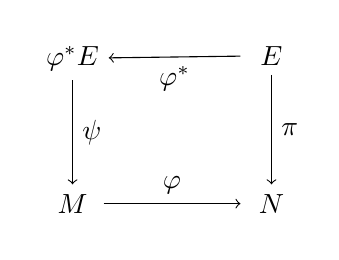
\begin{tikzpicture}
\matrix (m) [matrix of math nodes, row sep=3.8em, column sep=4.8em, minimum width=2.2em]
{
	\varphi^* E &  E  \\
	M  &  N  \\
};
\path[->]
(m-1-2) edge node [auto] {$ \varphi^*  $} (m-1-1)
edge node [auto] {$ \pi $} (m-2-2)
(m-2-1) edge node [auto]  {$  \varphi $} (m-2-2)
(m-1-1) edge node [auto] {$\psi$} (m-2-1)
;
\end{tikzpicture}
\qquad \, 
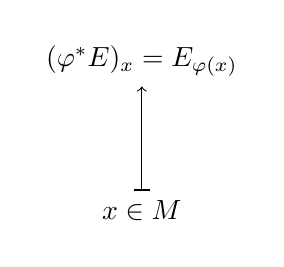
\begin{tikzpicture}
\matrix (m) [matrix of math nodes, row sep=3.8em, column sep=4.8em, minimum width=2.2em]
{
	(\varphi^* E)_x = E_{\varphi(x)}  \\
	 x\in M \\
};
 \path[|->]
	(m-2-1) edge node [auto] {$$} (m-1-1)
;
\end{tikzpicture}
\]
i.e. if $s\in \Gamma(E)$, 
\[
\varphi^* s = s \circ \varphi \in \Gamma( \varphi^* E)
\]
Thus,
\[
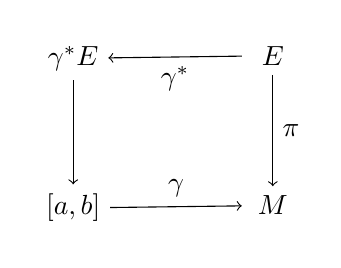
\begin{tikzpicture}
\matrix (m) [matrix of math nodes, row sep=3.8em, column sep=4.8em, minimum width=2.2em]
{
	\gamma^* E &  E  \\
	\left[a,b\right]  &  M  \\
};
\path[->]
(m-1-2) edge node [auto] {$ \gamma^*  $} (m-1-1)
edge node [auto] {$ \pi $} (m-2-2)
(m-2-1) edge node [auto]  {$  \gamma $} (m-2-2)
(m-1-1) edge node [auto] {$ $} (m-2-1)
;
\end{tikzpicture}
\qquad \, 
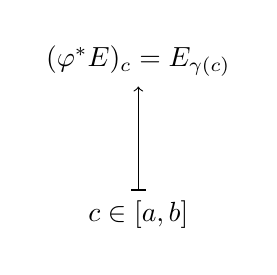
\begin{tikzpicture}
\matrix (m) [matrix of math nodes, row sep=3.8em, column sep=4.8em, minimum width=2.2em]
{
	(\varphi^* E)_c = E_{\gamma(c)}  \\
	 c\in  [a,b]\\
};
 \path[|->]
	(m-2-1) edge node [auto] {$$} (m-1-1)
;
\end{tikzpicture}
\]







For 
\[
\begin{gathered}
\dot{v}^k = -v^i \dot{s}^j \Gamma^k_{ \, \, ij}   \\
v^k(c) = v_0^k \qquad \, 1 \leq k \leq m
\end{gathered}
\]
\[
\dot{v} = -v^i \dot{s}^j \Gamma_{ij}
\]
\[
\begin{gathered}
\dot{ (v+w) } = -(v^i + w^i) \dot{s}^j \Gamma_{ij}
(v+w)(c) = v(c) + w(c) = v_0 + w_0 
\end{gathered}
\]
so $v+w\in \mathfrak{X}(s)$ is parallel transport of $v_0 + w_0$.  

Likewise, $\forall \, a \in \mathbb{F}$, $av \in \mathfrak{X}(s)$ is the parallel transport of $av_0$.  

\[
\dot{\mu}^k = - \mu^i \dot{s}^{\mu} \omega^k_{ \, \, i \mu} = -\mu^i \omega^k_{ \,\, i}(\dot{s}^{\mu})
\]


Suppose $\gamma^*E$ trivialized over $[a,b]$.  

Closed interval is contractible, so this is always possible.  

For chart $(U,\varphi)$, 
\[
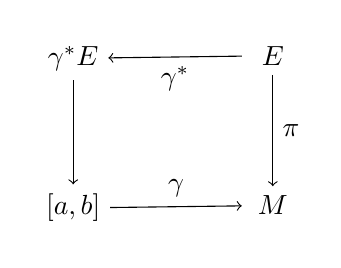
\begin{tikzpicture}
\matrix (m) [matrix of math nodes, row sep=3.8em, column sep=4.8em, minimum width=2.2em]
{
	\gamma^* E   &  E    \\
	\left[a,b\right]  &  M  \\
};
\path[->]
(m-1-2) edge node [auto] {$ \gamma^*  $} (m-1-1)
edge node [auto] {$ \pi $} (m-2-2)
(m-2-1) edge node [auto]  {$  \gamma $} (m-2-2)
(m-1-1) edge node [auto] {$ $} (m-2-1)
;
\end{tikzpicture} \qquad \, 
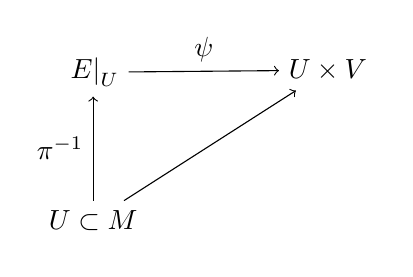
\begin{tikzpicture}
\matrix (m) [matrix of math nodes, row sep=3.8em, column sep=4.8em, minimum width=2.2em]
{
	\left. E \right|_U   &   U\times V  \\
	U \subset M    &    \\
};
\path[->]
(m-2-1) edge node [auto] {$ \pi^{-1}  $} (m-1-1)
edge node [auto] {$  $} (m-1-2)
(m-1-1) edge node [auto]  {$  \psi $} (m-1-2)
%(m-1-1) edge node [auto] {$ $} (m-2-1)
;
\end{tikzpicture}
\]
Consider 
\[
\begin{aligned}
& \varphi:[a,b]  \times V \to \gamma^* E \\ 
& \varphi(t,\cdot ) = \gamma^* \circ \psi^{-1}(\gamma(t), \cdot ) 
\end{aligned}
\]
$\forall \, \mu \in \Gamma( \left. E\right|_{x\in M} )$, \\ 
$\mu = \mu^i e_i$.  

$\varphi(t,e_i) = \epsilon_i$ is a basis for $\gamma^* E$.  

$\forall \, \sigma \in \Gamma(\gamma^*E)$,  
\[
\sigma  = \sigma^i \epsilon_i, \quad \, \sigma^i: [a,b] \to \mathbb{F}
\]
\[
\begin{gathered}
	\nabla_{ \frac{ \partial }{ \partial x^{\mu} } } \sigma = \frac{ \partial \sigma^k}{ \partial x^{\mu}  } \epsilon_k + \omega^k_{ \, \, j \mu } \sigma^j \epsilon_k = \left( \frac{ \partial \sigma ^k }{ \partial x^{\mu } } + \omega^k_{ \ , \, j \mu} \sigma^j  \right)  \epsilon_k \\ 
 \nabla \sigma = \epsilon_k \otimes ( d\sigma^k + \omega^k_{ \, \, j \mu} dx^{\mu} \sigma^j ) = \epsilon_k \otimes (d\sigma^k + \omega^k_{ \, \, j} \sigma^j  )  \\
 \nabla_{ \frac{d}{dt} } \sigma = \epsilon_k \otimes \left( \frac{d\sigma^k }{ dt } + \omega^k_{ \, \, j \mu } \dot{x}^{\mu} \sigma^j  \right)
\end{gathered}
\]
Now
\[
\frac{d}{dt} = \dot{x}^{\nu} \frac{ \partial }{ \partial x^{\nu } }
\]
Then $\sigma$ parallel along $\gamma$ if 
\[
\frac{ d\sigma^k}{ dt} + \omega^k_{ \, \, j\mu} \dot{x}^{\mu} \sigma^j = 0 
\]
\begin{definition}[3.1.4 \cite{ClSa2012}]  Parallel transport along $\gamma$ is 
\begin{equation}
\begin{aligned}
	& P_{\gamma} : E_{\gamma(a)} \to E_{\gamma(b)} \\ 
	& P_{\gamma}(v) \mapsto \sigma(b)
\end{aligned}
\end{equation}
where $\sigma \in \Gamma(\gamma^*E)$, $\sigma$ unique and s.t. $\sigma(a)=v$.  
\end{definition}







\begin{lemma}[10.1.16\cite{Conl2008}]
	holonomy 
	\[
	h_s:T_xM \to T_{x_0}M
	\]
	if $\nabla$ around piecewise smooth loop $s$ is a linear transformation.  
\end{lemma}






\begin{lemma}[10.1.18 Conlon (2008)\cite{Conl2008}] 
	Let piecewise smooth loop $s:[a,b] \to M$ at $x_0$.  

Let weak reparametrization $\widetilde{s} = s\circ r: [c,d] \to M$.  

If reparametrization is orientation-preserving, then $h_{\widetilde{s}} = h_s$, \\
If reparametrization is orientation-reversing, then $h_{\widetilde{s}} = h^{-1}_s$, 

\end{lemma}
\begin{proof}
	Without loss of generality,  assume smooth $s,r$
\[
\begin{aligned}
	& \widetilde{s}(\tau) = s(r(\tau)) \\ 
	& \widetilde{v}(\tau) = v(r(\tau))
\end{aligned}
\]
\[
\begin{aligned}
	& \widetilde{u}^j(\tau) = \frac{dt}{d\tau}(\tau) u^j(r(\tau)) \\ 
	& \frac{d\widetilde{v}^k}{d\tau} (\tau) = \frac{dr}{d\tau}(\tau) \frac{dv^k}{dt}(r(\tau)) \\ 
	& \frac{d\widetilde{v}^k }{ d\tau} = -\widetilde{v}^i \widetilde{u}^j \Gamma^k_{ij} 
\end{aligned}
\]
since \[
\begin{gathered}
	\frac{dv^k}{dt} = -v^i u^j \Gamma^k_{ij} ; \qquad \, 1\leq k \leq n \\ 
v^k(c) = a^k; \qquad \, 1\leq k \leq a 
\end{gathered}
\]
\[
\frac{dr}{d\tau} \frac{dv^k}{ dt} = -v^i \frac{dr}{d\tau} u^j \Gamma^k_{ \, \, ij} = \frac{d\widetilde{v}^k}{d\tau} = -\widetilde{v}^i \widetilde{u}^j \Gamma^k_{ \, \, ij}
\]
Thus, if $r(c) = a$, $r(d)=b$
\[
h_{\widetilde{s}}(v_0) = \widetilde{v}(d) = v(b) = h_s(v_0)
\]
If $r(c)=a$, $r(d)=b$, then 
\[
\widetilde{v}(c) = v(b) = h_s(v_0)
\]
and 
\[
h_{\widetilde{s}}(h_s(v_0)) = h_{\widetilde{s}}(v(b)) = \widetilde{v}(d) = v(a) = v_0
\]
At this point, I will switch to my notation because it clarified to me, at least, what was going on, in that a holonomy $h_s$ is \emph{invariant} under orientation-preserving reparametrization, and its inverse is well-defined.  

For $\widetilde{s} = s\circ t:[c,d] \to M$, \\
piecewise smooth $t$ is reparametrized, i.e. 
\begin{equation}
	t:[c,d] \to [a,b]
\end{equation}  
Now, 
\[
\begin{gathered}
	\frac{d}{d\tau}\widetilde{s}(\tau) = \frac{d}{d\tau} \widetilde{s}(t(\tau)) = \dot{s}(t) \frac{dt}{d\tau}(\tau) \equiv \dot{s} \frac{dt}{d\tau} \\ 
v^k(t) = v^k(t(\tau)) = v^k(\tau) \\ 
 \frac{dv^k}{d\tau}(t(\tau) ) = \frac{dv^k}{dt} \frac{dt}{ d\tau } = \frac{dt}{d\tau}(-v^i( \tau) \dot{s}^j(t) \Gamma^k_{ \,\, ij} ) = -v^i(\tau) \frac{d\widetilde{s}^j }{ d\tau} \Gamma^k_{ \, \, ij} 
\end{gathered}
\]
Consider 
\[
h_s(v_0) = v(b)
\]
If $\begin{aligned} & \quad \\ 
	& t(c) = a \\ 
	& t(d)=b \end{aligned}$, 
\[
h_{\widetilde{s}}(v_0) = \widetilde{v}(d) = v(t(d)) = v(b) = h_s(v_0)
\]
If $\begin{aligned} & \quad \\ 
	& t(c) = b \\ 
	& t(d)=a \end{aligned}$, 
\[
\begin{gathered}
h_{\widetilde{s}}(h_s(v_0) )  = h_{\widetilde{s}}( v(b)) = h_{\widetilde{s}}(v(t(c))) = h_{\widetilde{s}}(\widetilde{v}(c)) = \\
	= \widetilde{v}(d) = v(t(d)) = v(a) = v_0
\end{gathered}
\]
Thus, 
\[
\boxed{ h_{\widetilde{s}}= h_s^{-1} }
\]


\end{proof}

I am working through Conlon (2008) \cite{Conl2008} , Clarke and Santoro (2012) \cite{ClSa2012}, and Schreiber and Waldorf (2007) , concurrently, for holonomy.  









\part{Complex Manifolds}

EY : 20170123 I don't see many good books on Complex Manifolds for physicists other than Nakahara's.  I will supplement this section on Complex Manifolds with external links to the notes of other courses that I found useful to myself.


\href{http://www.caramdir.at/uploads/math/piii-cm/complex-manifolds.pdf}{Complex Manifolds - Lecture Notes}
Koppensteiner (2010) \cite{Kopp2010}


\href{http://www.staff.science.uu.nl/~vando101/MRIlectures.pdf}{Lectures on Riemannian Geometry, Part II: Complex Manifolds by Stefan Vandoren}

Vandoren (2008) \cite{Vand2008}

\part{Jets, Jet bundles, $h$-principle, $h$-Prinzipien}

cf. Eliashberg and Misahchev (2002) \cite{ElMi2002}

cf. Ch. 1 Jets and Holonomy, Sec. 1.1 Maps and sections of Eliashberg and Misahchev (2002) \cite{ElMi2002}.  

Visualize $f:\mathbb{R}^n \to \mathbb{R}^q$ as graph $\Gamma_f \subset \mathbb{R}^n \times \mathbb{R}^q$.  

Consider this graph as image of $\begin{aligned} & \quad \\ 
	& \mathbb{R}^n \to \mathbb{R}^n \times \mathbb{R}^q \\
	& x \mapsto (x,f(x)) \end{aligned}$, i.e. 

$\begin{aligned} & \quad \\ 
	& \mathbb{R}^n \to \mathbb{R}^n \times \mathbb{R}^q \\
	& x \mapsto (x,f(x)) \end{aligned}$ is called section (by mathematicians), \\
is called \emph{field} or $\mathbb{R}^q$-valued field (by physicists).  

cf. Ch. 1 Jets and Holonomy, Sec. 1.2 Coordinate definition of jets of Eliashberg and Misahchev (2002) \cite{ElMi2002}.  

\begin{definition}[$r$-jet]
Given (smooth) $f: \mathbb{R}^n \to \mathbb{R}^q$, given $x\in \mathbb{R}^n$.  

$r$-jet of $f$ at $x$ - sequence of derivatives of $f$, up to order $r$, $\equiv$ 
\begin{equation}
J^r_f(x) = (f(x),f'(x) \dots f^{(r)}(x) )
\end{equation}
\end{definition}

$f^{(q)}$ consists of all partial derivatives $D^{\alpha}f$, $\alpha= (\alpha_1\dots \alpha_n)$, $|\alpha| = \alpha_1 + \dots + \alpha_n =s$, ordered lexicographically.  

e.g. $q=1$, \\
$f: \mathbb{R}^n \to \mathbb{R}$.   \\
1-jet of $f$ at $x = J_f^1(x) = (f(x), f^{(1)}(x))$.  
\[
f^{(1)}(x) = \lbrace D^{\alpha}f| \alpha = (\alpha_1 \dots \alpha_n), |\alpha| = \alpha_1  + \dots + \alpha_n  =1 \rbrace = \left( \frac{ \partial f}{ \partial x^1 }, \frac{ \partial f}{ \partial x^2 } , \dots \frac{ \partial f}{ \partial x^n } \right)
\]
Let $d_r = d(n,r) = $ number of all partial derivatives $D^{\alpha}$ of order $r$ of function $\mathbb{R}^n \to \mathbb{R}$.  

Consider $r$-jet $J^r_f(x)$ of map $f:\mathbb{R}^n\to \mathbb{R}^q$ as pt. of space $\mathbb{R}^q \times \mathbb{R}^{qd_1} \times \mathbb{R}^{qd_2} \times \dots \times \mathbb{R}^{qd_r} = \mathbb{R}^{q N_r}$, where $N_r = N(n,r) = 1 + d_1 + d_2 + \dots + d_r$, i.e. 
\[
J_f^r(x) = (f(x),f^{(1)}(x) , \dots f^{(r)}(x) ) \in \mathbb{R}^q \times \mathbb{R}^{qd_1} \times  \dots \times \mathbb{R}^{qd_r} = \mathbb{R}^{q N_r}
\]


\exercisehead{1}  

Given order $r$, consider $n$-tuple of (positive) integers $(r_1,r_2\dots r_n)$ s.t. $r_1 + r_2 + \dots + r_n = r$, and $r_k\geq 0$. \\
 Imagine $r_k = $ occupancy number, num ber of balls in $k$th cell.  $(r_1\dots r_n)$ describes a positive ocnfiguration of occupancy numbers, with indistinguishable balls; 2 distributions are distinguishable only if corresponding $n$-tuples $(r_1 \dots r_n)$ not identical.  

Represent balls by stars, and indicate $n$ cells by $n$ spaces between $n+1$ bars.  

With $n+1$ bars, $r$ stars, 2 bars are fixed. $n-1$ bars and $r$ stars to arrange linearly, so a total of $n-1+r$ objects to arrange.  $r$ stars indistinguishable amongst themselves, so choose $r$ out of $n-1+r$ to be stars.  
\begin{equation}
\Longrightarrow d_r = d(n,r)=\binom{n-1+r}{r}
\end{equation}

Use \emph{induction} (cf. \href{http://www.cs.columbia.edu/~cs4205/files/CM4.pdf}{Ch. 4 Binomial Coefficients}).  
\[
\begin{aligned}
	& N_0 = N(n,0) = \binom{n-1+0}{0} = 1 \\ 
	& N_1 = N(n,1) = 1+ \binom{n-1+1}{1} = 1 + n = \frac{ (n+1)!}{n! 1!}
\end{aligned}
\]
Induction step: 
\[
N_{r-1} = N(n,r-1) = \sum_{k=1}^{r-1} d_k + 1 = \binom{ n+r-1}{r-1}
\]
and so 
\[
\begin{gathered}
N_r = N(n,r) = \sum_{k=1}^r d_k + 1 = \sum_{k=1}^r \binom{n-1+k}{k} + 1 = \sum_{k=1}^{r-1} \binom{ n-1 +k}{k} + \binom{n-1+r}{r} + 1 = \\
	 =  \binom{n+r-1}{r-1} + \binom{n-1+r}{r} = \frac{ (n+r-1)! }{ (r-1)! n!} + \frac{ (n-1+r)! }{ r! (n-1)! } = \frac{ (n+r)!}{n!r!} = \binom{n+r}{r}
\end{gathered}
\]
\[
\begin{tikzpicture}
  \matrix (m) [matrix of math nodes, row sep=3.8em, column sep=4.8em, minimum width=2.2em]
  {
    \mathbb{R}^{qN_r} &  \\ 
    \mathbb{R}^n & \mathbb{R}^q \\ 
};
  \path[->]
  (m-2-1) edge node [auto] {$ J_f^r $} (m-1-1)
          edge node [auto] {$f $} (m-2-2)
  ;
\end{tikzpicture}   \quad \quad \, \begin{tikzpicture}
  \matrix (m) [matrix of math nodes, row sep=3.8em, column sep=4.8em, minimum width=2.2em]
  {
   J_f^r(x)  &  \\ 
    x & f(x) \\ 
};
  \path[|->]
  (m-2-1) edge node [auto] {$ J_f^r $} (m-1-1)
          edge node [auto] {$f $} (m-2-2)
  ;
\end{tikzpicture}  
\]

\begin{definition}[space of $r$-jets]
space of $r$-jects of maps $\mathbb{R}^n \to \mathbb{R}^q$ or space of $r$-jets of sections $\mathbb{R}^n \to \mathbb{R}^n \times \mathbb{R}^q \equiv $
\begin{equation}
J^r(\mathbb{R}^n, \mathbb{R}^q) = \mathbb{R}^n \times \mathbb{R}^{qN_r} \equiv \mathbb{R}^n \times \mathbb{R}^q \times \mathbb{R}^{qd_1} \times \mathbb{R}^{qd_2} \times \dots \times \mathbb{R}^{qd_r}
\end{equation}
e.g. $J^1(\mathbb{R}^n, \mathbb{R}^q) = \mathbb{R}^n \times \mathbb{R}^q \times M_{q\times n}$, where $M_{q\times n} = \mathbb{R}^{qn}$ is the space of $(q\times n)$-matrices.  
\end{definition}


\part{Morse Theory}

\section{Morse Theory introduction from a physicist}

I needed some physical motivation to understand Morse theory, and so I looked at Hori, et. al. \cite{Hori2003}.  

cf. pp. 43, Sec. 3.4 Morse Theory, from Ch. 3. Differential and Algebraic Topology of Hori, et. al. \cite{Hori2003}.

Consider smooth $f:M \to \mathbb{R}$, with non-degenerate critical points.

If no critical values of $f$ between $a$ and $b$ ($a<b$), then subspace on which $f$ takes values less than $a$ is deformation retract of subspace where $f$ less than $b$, i.e.
\[
\lbrace x \in M | f(x) < b\rbrace \times [0,1] \xrightarrow{ F } \lbrace x \in M | f(x) < b\rbrace
\]
$\forall \, x \in M$ s.t. $f(x) < b$,
\[
\begin{aligned}
  & F(x,0)  = x \\
  & F(x,1) \in \lbrace x \in M | f(x) < a \rbrace 
  \end{aligned} \qquad \qquad \, \text{ and } F(a',1) = a' \qquad \, \forall \, a' \in M \text{ s.t. } f(a') < a
\]

To show this, consider $-\nabla f/|\nabla f|^2$

Morse lemma: $\forall \, $ critical pt. $p$ s.t. $\exists \, $ choice of coordinates s.t.
\begin{equation}
  f  = - (x_1^2 + x_2^2 + \dots + x_{\mu}^2) + x_{\mu + 1}^2 + \dots + x_n^2
\end{equation}
where $f(p)=0$ and $p$ is at origin of these coordinates.

\begin{itemize}
\item difference between
  \[
f^{-1}(\lbrace x \leq -\epsilon \rbrace) , \, f^{-1}(\lbrace x \leq + \epsilon \rbrace)
\]
can be determined by local analysis and only depends on $\mu$, $\mu \equiv $ ``Morse index'' $=$ number of negative eigenvalues of Hessian of $f$ at critical pt.

Answer: \\

\[
f^{-1}(\lbrace x \leq + \epsilon \rbrace) \text{ can be obtained from } f^{-1}(\lbrace x \leq -\epsilon \rbrace) \text{ by ``attaching $\mu$-cell'' along boundary $f^{-1}(0)$ }
\]

\item ``attaching $\mu$-cell to $X$ mean, take
  $\mu$-ball $B_{\mu} = \lbrace |x| \leq 1 \rbrace$ in $\mu$-dim. space, \\
  identity pts. on boundary $S^{\mu-1}$ with pts. in the space $X$, through \\
  cont. $f : S^{\mu-1} \to X$, i.e. take
  \[
X \coprod B_{\mu}
\]
with $x\sim f(x)$ \, $\forall \, x \in \partial B_{\mu} = S^{\mu -1}$.

 
\item find homology of $M$,
  
  $f$ defines chain complex $C_f^*$, $k$th graded piece $C^{\alpha_k}$, $\alpha_k$ is number of critical pts. with index $k$.
  \begin{equation}
\begin{aligned}
  & \partial : C_p^k \to C^{k-1}_p \\ 
  & \partial x_a = \sum_b \Delta_{a,b} x_b 
  \end{aligned}
    \end{equation}
  where $\Delta_{a,b} :=$ signed number of lines of gradient flow from $x_a$ to $x_b$, $b$ labels pts. of index $k-1$.

  Gradient flow line is path $x(t)$ s.t. $\dot{x} = \nabla (f)$, with $\begin{aligned} & \quad  \\
    & x(-\infty) = x_a \\
    & x(+\infty) = x_b \end{aligned}$

\item  To define this number ($\Delta_{a,b} $?), construct moduli space of such lines of flow (???) \\
  by intersecting outward and inward flowing path spaces from each critical point, and then show this moduli space is oriented, 0-dim. manifold (pts. with signs)

\item $\partial^2=0$ proof

  $\partial$, boundary of space of paths connecting critical points, whose index differs by $2 =$ union over compositions of paths between critical pts. whose index differs by $1$.

  $\Longrightarrow$ coefficients of $\partial^2$ are sums of signs of pts. in $0$-dim. space, which is boundary of $1$-dim. space.

  These signs must therefore add to $0$, so $\partial^2=0$.  
  
  \end{itemize}

Hori, et. al. \cite{Hori2003} is good for physics, but there isn't much thorough, step-by-step explanations of the math.  I will look at Hirsch (1997) \cite{MHirsch1997} and Shastri (2011) \cite{AShastri2011} at the same time.  

\subsection{Introduction, definitions of Morse Functions, for Morse Theory}

cf. Ch. 6, Morse Theory of Hirsch (1997) \cite{MHirsch1997}, Section 1. Morse Functions, pp. 143-

Recall for $TM$, $T_xM \xrightarrow{\varphi}\mathbb{R}^n$.  \\
Cotangent bundle $T^*M$ defined likewise:
\[
T^*_xM \xrightarrow{ \varphi } \text{ dual vector space } (\mathbb{R}^n)^* = L(\mathbb{R}^n,\mathbb{R})
\]
i.e.
\[
T^*M = \bigcup_{x\in M} (M_x^*) \qquad \qquad \, M_x^* = L(M_x,\mathbb{R})
\]
If chart $(\varphi, U)$ on $M$, natural chart on $T^*M$ is
\[
\begin{aligned}
  & T^*U \to \varphi(U) \times (\mathbb{R}^n)^* \\ 
  & \lambda \in M_x^* \mapsto (\varphi(x), \lambda \varphi_x^{-1} )
  \end{aligned}
\]

Projection map
\[
\begin{aligned}
  & p : T^* \to M \\ 
  & M_x^* \mapsto x
  \end{aligned}
\]
Let $C^{r+1}$ map, $1\leq r \leq \omega$, $f:M \to \mathbb{R}$, $\forall \, x \in M$, linear map $T_x f :M_x \to \mathbb{R}$ belongs to $M_x^*$
\[
T_xf = Df_x \in M_x^*
\]
Then
\[
\begin{aligned}
  & Df:M \to T^*M \\ 
  &  x\mapsto Df_x = Df(x)
  \end{aligned}
\]
is $C^r$ section of $T^*M$.  

\begin{definition}
  \textbf{critical point} $x$ of $f$ is zero of $Df$, i.e. \begin{equation}
Df(x) = 0 
  \end{equation} of vector space $M_x^*$.  
  \end{definition}

Thus, set of critical pts. of $f$ is counter-image of submanifold $Z^* \subset T^*M$ of zeros.  \\
Note $Z^*\approx M$, codim. of $Z^*$ is $n=\text{dim}M$.  

\begin{definition}
  \textbf{Morse function} $f$ if $\forall \, $ critical pts. of $f$ are nondegenerate.
  \end{definition}

Note set of critical pts. closed discrete subset of $M$.  \\
Let open $U \subset \mathbb{R}^n$, let $C^2$ map $g:U\to \mathbb{R}$, \\
critical pt. $p\in U$ nondegenerate iff
\begin{itemize}
\item linear $D(Dg)(p):\mathbb{R}^n \to (\mathbb{R}^n)^*$ bijective
\item identify $L(\mathbb{R}^n, (\mathbb{R}^n)^*)$ with space of bilinear maps $\mathbb{R}^n \times \mathbb{R}^n \to \mathbb{R}$, $\Longrightarrow$ equivalent to condition that symmetric bilinear $D^2g(p) : \mathbb{R}^n \times \mathbb{R}^n \to \mathbb{R}$ non-degenerate 
\item $n\times n$ \emph{Hessian matrix}
  \[
\left[ \frac{ \partial^2 g}{ \partial x^i  \partial x^j }(p) \right]
\]
has rank $n$
\end{itemize}

Hessian of $g$ at critical pt. $p$ is quadratic form $H_pf$ associated to bilinear form $D^2g(p)$
\[
\Longrightarrow H_pf(y) =D^2g(p)(y,y) = \sum_{i,j} \frac{ \partial^2g}{ \partial x^i \partial x^j}(p)y^i y^j
\]

Let open $V \subset \mathbb{R}^n$, suppose $C^2$ diffeomorphism $h: V\to U$.

Let $q=h^{-1}(p)$, so $q$ is critical pt. of $gh:V\to \mathbb{R}$.

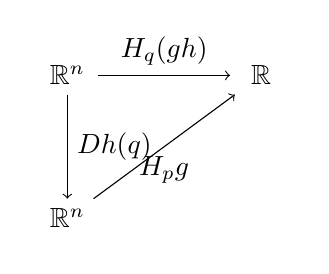
\begin{tikzpicture}
  \matrix (m) [matrix of math nodes, row sep=3.8em, column sep=4.8em, minimum width=2.2em]
  {
    \mathbb{R}^n & \mathbb{R} \\ 
     \mathbb{R}^n & \\ 
};
  \path[->]
  (m-1-1) edge node [above] {$H_q(gh) $} (m-1-2)
          edge node [auto] {$Dh(q) $} (m-2-1)
  (m-2-1) edge node [below] {$H_pg $} (m-1-2)
  ;
\end{tikzpicture}  

(quadratic) form $(H_pf)$ invariant under diffeomorphisms.


Let $C^2$ $f:M\to \mathbb{R}$.  \\
$\forall \,$ critical pt. $x$ of $f$, define \\
Hessian quadratic form
\[
\begin{aligned}
  & H_xf : M_x \to \mathbb{R} \\ 
  & H_xf : M_x \xrightarrow{ D\varphi_x } \mathbb{R}^n \xrightarrow{ H_{\varphi(x)}(f\varphi^{-1} ) } \mathbb{R}
\end{aligned}
\]
where $\varphi$ is any chart at $x$.

Thus, critical pt. of a $C^2$ real-valued function nondegenerate iff associated Hessian quadratic form is nondegenerate.  

Let $Q$ nondegenerate quadratic form on vector space $E$.

$Q$ negative definite on subspace $F \subset E$ if $Q(x)<0$ whenever $x\in F$ nonzero.

Index of $Q \equiv \text{Ind}Q$, is largest possible dim. of subspace on which $Q$ is negative definite.








cf. 1.1. Morse's Lemma of  Ch. 6, pp. 145, Morse Theory of Hirsch (1997) \cite{MHirsch1997}

\begin{lemma}[Morse's Lemma]
  Let $p\in M$ be nondegenerate critical pt. of index $k$ of $C^{r+2}$ map $f:M\to \mathbb{R}$, $1\leq r \leq \omega$.

  Then $\exists \, C^r$ chart $(\varphi,U)$ at $p$ s.t.
  \begin{equation}
    f\varphi^{-1}(u_1 \dots u_n) = f(p) - \sum_{i=1}^k u_i^2 + \sum_{i = k+1}^n u_i^2
  \end{equation}
  \end{lemma}

Let ${\,}^TQ \equiv Q^T$ denote tranpose of matrix $Q$.

\begin{lemma}
  Let $A = \text{diag}\lbrace a_1 , \dots , a_n \rbrace$ diagonal $n\times n$ matrix, with diagonal entries $\pm 1$.

  Then $\exists \, $ neighborhood $N$ of $A$ in vector space of symmetric $n\times n$ matrices, $C^{\infty}$ map
  \begin{equation}
P:N \to GL(n,\mathbb{R})
  \end{equation}
  s.t. $P(A)=I$, and if $P(B) = Q$, then $Q^T BQ = A$
\end{lemma}

\begin{proof}
  Let $B = [b_{ij}]$ be symmetri matrix near $A$ s.t. $b{11} \neq 0$ and $b_{11}$ has same sign as $a_1$.

    Consider $x=Ty$ where
    \[
\begin{aligned}
&  x_1 = \left[ y_1 - \frac{b_{12}}{b_{11}} y_2 - \dots - \frac{b_{1n}}{b_{11}} y_n \right] / \sqrt{ |b_n | } \\ 
& x_k = y_k \text{ for } k = 2, \dots n 
  \end{aligned}
    \]
  \end{proof}


\section{Lagrange multipliers}

From \emph{wikipedia:Lagrange multiplier}, \url{https://en.wikipedia.org/wiki/Lagrange_multiplier},
find local minima (maxima), pt. $a\in N$, s.t. $\exists \, $ neighborhood $U$ s.t. $f(x) \geq f(a)$ ($f(x) \leq f(a)$) \, $\forall \, x\in U$.

For $f:U\to \mathbb{R}$, open $U\subset \mathbb{R}^n$, find $x\in U$ s.t. $D_xf \equiv Df(x) =0$, check if Hessian $H_x f<0$.

Maxima may not exit since $U$ open.


References:

\href{http://www.math.uni.wroc.pl/~karch/analiza_nieliniowa/18_mnozniki-lagrangea.pdf}{Relative Extrema and Lagrange Multipliers}

Other interesting links:

\href{http://oai.cwi.nl/oai/asset/2552/2552A.pdf}{The Lagrange Multiplier Rule on Manifolds and Optimal Control of nonlinear systems}


\part{Classical Mechanics applications}

cf. Arnold, Kozlov, Neishtadt (2006) \cite{AKN2006}. 

If known forces $\mathbf{F}_1 \dots \mathbf{F}_n$ acts on points, then 
\begin{equation}
\sum_{i=1}^n \langle m_i \ddot{ \mathbf{r}}_i - \mathbf{F}_i , \mathbf{\xi}_i \rangle = 0
\end{equation}
cf. Eq. (1.26) of Arnold, Kozlov, Neishtadt (2006) \cite{AKN2006}, where $\xi_1 , \dots \xi_n$ are arbitrary tangent vectors to $M$, $\mathbf{\xi}_i, \dots \mathbf{\xi}_n \in TM$.  

$\sum_{i=1}^n \langle m_i \ddot{ \mathbf{r}}_i - \mathbf{F}_i , \mathbf{\xi}_i \rangle$ called "general equation of dynamics" or d'Alembert-Lagrange principle.  







\end{multicols*}

\begin{thebibliography}{9}

\bibitem{Fell1968}
William Feller.  \textbf{An Introduction to Probability Theory and Its Applications}, Vol. 1, 3rd Edition.  1968.  ISBN-13: 978-0471257080



\bibitem{JLee2009}
Jeffrey M. Lee. \textbf{Manifolds and Differential Geometry}, \emph{Graduate Studies in Mathematics} Volume: 107, American Mathematical Society, 2009. ISBN-13: 978-0-8218-4815-9

\bibitem{JLee2012}
John Lee, \textbf{Introduction to Smooth Manifolds} (Graduate Texts in Mathematics, Vol. 218), 2nd edition, Springer,  2012, ISBN-13: 978-1441999818

\bibitem{VGuilleminAPollack2010}
Victor Guillemin, Alan Pollack. \textbf{Differential Topology}. American Mathematical Society. 2010. ISBN-13: 978-0821851937
\url{https://www.google.com/url?sa=t&rct=j&q=&esrc=s&source=web&cd=2&cad=rja&uact=8&ved=0ahUKEwjG96q9z63JAhWMLYgKHempDoMQFggmMAE&url=http\%3A\%2F\%2Fwww.mat.unimi.it\%2Fusers\%2Fdedo\%2Ftop\%2520diff\%2FGuillemin-Pollack_Differential\%2520topology.pdf&usg=AFQjCNF5imOH5xeXRSK60qzM7zT97sdIsw}

\bibitem{AShastri2011}
Anant R. Shastri. \textbf{Elements of Differential Topology}. CRC Press. 2011. ISBN-13: 978-0415339209

\bibitem{MHirsch1997}
Morris W. Hirsch, \textbf{Differential Topology} (Graduate Texts in Mathematics), Graduate Texts in Mathematics (Book 33), Springer (September 16, 1997). ISBN-13: 978-0387901480

\bibitem{Pras1996}
Agostino Pr\'{a}staro.  \textbf{Geometry of PDEs and Mechanics}.  World Scientific Publishing Co.  1996.  QC125.2.P73 1996  530.1'55353--dc20.  

Agostino Pr\'{a}staro.  \emph{Dipartimento di Metodi e Modelli Matematici per le Scienze Applicate, Universit\`{a} degli Studi di Roma ``La Sapienza''}.  

\bibitem{Kopp2010}
  Clemens Koppensteiner.  \emph{Complex Manifolds: Lecture Notes}.  \url{http://www.caramdir.at/uploads/math/piii-cm/complex-manifolds.pdf}
  

\bibitem{Vand2008}
Stefan Vandoren. \textbf{Lectures on Riemannian Geometry, Part II: Complex Manifolds}.  \url{http://www.staff.science.uu.nl/~vando101/MRIlectures.pdf} 

\bibitem{Hori2003}
Kentaro Hori (Author, Editor), Sheldon Katz (Editor), Albrecht Klemm (Editor), Rahul Pandharipande (Editor), Richard Thomas (Editor), Cumrun Vafa (Editor), Ravi Vakil (Editor), Eric Zaslow (Editor).  \textbf{Mirror Symmetry} (Clay Mathematics Monographs, V. 1).  Clay Mathematics Monographs (Book 1).  American Mathematical Society (August 19, 2003).  ISBN-10: 0821829556  ISBN-13: 978-0821829554  \url{https://web.archive.org/web/20060919020706/http://math.stanford.edu/~vakil/files/mirrorfinal.pdf}

\bibitem{Conl2008}
Lawrence Conlon.  \textbf{Differentiable Manifolds} (Modern Birkhäuser Classics).  2nd Edition.  Birkhäuser; 2nd edition (October 10, 2008).  ISBN-13: 978-0817647667




\bibitem{ClSa2012}
Andrew Clarke and Bianca Santoro.  \emph{Holonomy Groups in Riemannian Geometry}.  \href{https://arxiv.org/pdf/1206.3170.pdf}{arXiv:1206.3170 [math.DG]}

\bibitem{ScWa2007}
Urs Schreiber and Konrad Waldorf.  \emph{Parallel Transport and Functors}.  \href{https://arxiv.org/pdf/0705.0452.pdf}{arXiv:0705.0452 [math.DG]}

\bibitem{ElMi2002}
Y. Eliashberg, N. Mishachev, \emph{Introduction to the $h$-principle}, Grad. Studies in Math. Vol 48 (AMS 2002)


\bibitem{AKN2006}
Vladimir I. Arnold, Valery V. Kozlov, Anatoly I. Neishtadt.  \textbf{Mathematical Aspects of Classical and Celestial Mechanics}.  Third Edition.  Springer.  


\end{thebibliography}


\end{document}
